%%
% A header that lets you compile a chapter by itself, or inside a larger document.
% Adapted from http://stackoverflow.com/questions/3655454/conditional-import-in-latex
%
%
%Use \inbpdocument and \outbpdocument in your individual files, in place of \begin{document} and \end{document}. In your main file, put in a \def \ismaindoc {} before including or importing anything.
%
% David Duvenaud
% June 2011
% 
% ======================================
%
%


\ifx\ismaindoc\undefined
	\newcommand{\inbpdocument}{
		\def \ismaindoc {}
		% Use this header if we are compiling by ourselves.
		\documentclass[a4paper,11pt]{common/PhDThesisPSnPDF}
		\usepackage[round]{natbib} 
\usepackage{hyperref} 
\usepackage{url} %tablerules
\usepackage{cleveref}
\usepackage{soul}


%\usepackage{draftwatermark}
%\SetWatermarkLightness{0.95}

% ******************************************************************************
% ****************************** Custom Margin *********************************

% Add `custommargin' in the document class options to use this section
% Set {innerside margin / outerside margin / topmargin / bottom margin}  and
% other page dimensions

\ifsetMargin
\else
    \RequirePackage[left=37mm,right=30mm,top=35mm,bottom=30mm]{geometry}
    \setFancyHdr % To apply fancy header after geometry package is loaded
\fi


%\chead{Unfinished draft}
\cfoot{\texttt{Unfinished draft - compiled on \today{} at \currenttime}}

% *****************************************************************************
% ******************* Fonts (like different typewriter fonts etc.)*************

% Add `customfont' in the document class option to use this section

\ifsetFont
\else
    % Set your custom font here and use `customfont' in options. Leave empty to
    % load computer modern font (default LaTeX font).  

    \RequirePackage{libertine} 
\fi



% Add appendices
\RequirePackage[title,titletoc]{appendix}

% changes the default name `Bibliography` -> `References'
%\renewcommand{\bibname}{References}


% *****************************************************************************
% *************** Changing the Visual Style of Chapter Headings ***************
% Uncomment the section below. Requires titlesec package.

%\RequirePackage{titlesec}
%\newcommand{\PreContentTitleFormat}{\titleformat{\chapter}[display]{\scshape\Large}
%{\Large\filleft{\chaptertitlename} \Huge\thechapter}
%{1ex}{}
%[\vspace{1ex}\titlerule]}
%\newcommand{\ContentTitleFormat}{\titleformat{\chapter}[display]{\scshape\huge}
%{\Large\filleft{\chaptertitlename} \Huge\thechapter}{1ex}
%{\titlerule\vspace{1ex}\filright}
%[\vspace{1ex}\titlerule]}
%\newcommand{\PostContentTitleFormat}{\PreContentTitleFormat}
%\PreContentTitleFormat


% *****************************************************************************
% **************************** Custom Packages ********************************
% *****************************************************************************


% ************************* Algorithms and Pseudocode **************************

%\usepackage{algpseudocode} 


% ********************Captions and Hyperreferencing / URL **********************

% Captions: This makes captions of figures use a boldfaced small font. 
%\RequirePackage[small,bf]{caption}

\RequirePackage[labelsep=space,tableposition=top]{caption} 
\renewcommand{\figurename}{Fig.} %to support older versions of captions.sty
\captionsetup{belowskip=12pt,aboveskip=4pt}

% ************************ Formatting / Footnote *******************************

%\usepackage[perpage]{footmisc} %Range of footnote options 


% ****************************** Line Numbers **********************************

%\RequirePackage{lineno}
%\linenumbers

% ************************** Graphics and figures *****************************

\usepackage{rotating}
\usepackage{lscape} 
%\usepackage{wrapfig}
%\usepackage{float}
%subfigures deprecated
%\usepackage{subfigure}
%use subcaption instead
\usepackage[labelfont=bf,labelsep=period,justification=raggedright]{caption}
\usepackage{subcaption}
%\usepackage{subfig} %note: subfig must be included after the `caption` package. 


% ********************************* Table **************************************

%for table cell with diagonal division
%\usepackage{multicol}
\usepackage{multirow}
\usepackage{tabularx}
\usepackage{slashbox}
\usepackage{longtable} 
\usepackage{booktabs}
\usepackage{tabu}
\usepackage{xcolor,colortbl}



% ***************************** Math and SI Units ******************************

\usepackage{amsthm}
\usepackage{amsfonts}
\usepackage{amsmath}
\usepackage{amssymb}
\usepackage{textcomp}
% degree celsius
%\usepackage{gensymb}
%percentages, microliters, nanograms etc
\usepackage{siunitx}
\DeclareSIUnit[number-unit-product={}]\unit{U}


% ******************************************************************************
% ************************* User Defined Commands ******************************
% ******************************************************************************

% *********** To change the name of Table of Contents / LOF and LOT ************

%\renewcommand{\contentsname}{My Table of Contents}
%\renewcommand{\listfigurename}{My List of Figures}
%\renewcommand{\listtablename}{My List of Tables}


% ********************** TOC depth and numbering depth *************************

%\setcounter{secnumdepth}{2}
%\setcounter{tocdepth}{2}

% ******************************* Nomenclature *********************************

% To change the name of the Nomenclature section, uncomment the following line

%\renewcommand{\nomname}{Symbols}


% ********************************* Appendix ***********************************

% The default value of both \appendixtocname and \appendixpagename is `Appendices'. These names can all be changed via: 

%\renewcommand{\appendixtocname}{List of appendices}
%\renewcommand{\appendixname}{Appndx}


%%% Packages
% Use Charter font.
%\usepackage{charter}
% for line spacing
\usepackage{setspace}
\usepackage{xspace}
% Use PDF output.
%\usepackage[pdftex]{color,graphicx}
% The output should be wide.
%\usepackage{a4wide}
%\usepackage[a4paper]{geometry}
%\usepackage[text={7.5in,9in},centering]{geometry}
%\usepackage[cm]{fullpage}
%for definition list
\usepackage{enumitem}
%puts silly zeroes in section names
%\usepackage{fancyhdr}
%for code snippets
%\usepackage{float}
%\floatstyle{ruled}
%\newfloat{program}{thp}{lop}
%\floatname{program}{Code snippet} 
\usepackage{tikz}
\usetikzlibrary{shapes,arrows,calc,through,backgrounds,decorations.pathmorphing,shadows} 
%\usepackage[active,tightpage]{preview} 
\usepackage[french, greek, english]{babel}
%input encoding
%\usepackage[iso-8859-7]{inputenc}
%\usepackage[latin1]{inputenc}
%output encoding
\usepackage[T1]{fontenc}
\selectlanguage{english} 
% Pour la dedicace
\usepackage{frcursive} 
%side caption: SCfigure
%\usepackage{sidecap}
%\usepackage[table]{xcolor}
%\usepackage[graphics,tightpage,active]{preview}
%\PreviewEnvironment{tikzpicture}
%\PreviewEnvironment{equation}
%\PreviewEnvironment{equation*}
%\newlength{\imagewidth}
%\newlength{\imagescale}
%\pagestyle{empty}
%\thispagestyle{empty}
%\usepackage{standalone} 
\usepackage[section,subsection,subsubsection]{extraplaceins} 
\usepackage{authblk} 
\usepackage{graphicx} 
%unicode support
\usepackage[utf8]{inputenc} 
%multiple indices
\usepackage{multind}
%glossary
\usepackage[acronym]{glossaries}

\usepackage{datetime}
\renewcommand{\tabularxcolumn}[1]{>{\arraybackslash}m{#1}}
\usepackage{relsize}
\usepackage{nicefrac}
\usepackage{nth}
\usepackage{array}




		% All my custom preamble stuff.  Shouldn't overlap with anything in official-preamble


% Paths to figure and table directories.
\newcommand{\symmetryfigsdir}{figures/symmetries}
\newcommand{\topologyfiguresdir}{figures/topology}
\newcommand{\infinitefiguresdir}{figures/infinite}
\newcommand{\grammarfiguresdir}{figures/grammar}
\newcommand{\introfigsdir}{figures/intro}
\newcommand{\gplvmfiguresdir}{figures/gplvm}
\newcommand{\warpedfiguresdir}{figures/warped-mixtures}
\newcommand{\deeplimitsfiguresdir}{figures/deep-limits}
\newcommand{\quadraturefigsdir}{figures/quadrature}
\newcommand{\additivefigsdir}{figures/additive}
\newcommand{\decompfigsdir}{figures/decomp}
\newcommand{\examplefigsdir}{figures/worked-example}


\usepackage{bm}  % for warped mixtures - is this necessary?
\usepackage{booktabs}
\usepackage{tabularx}
\usepackage{multirow}
\usepackage{datetime}
\renewcommand{\tabularxcolumn}[1]{>{\arraybackslash}m{#1}}
\usepackage{relsize}
\usepackage{graphicx}
\usepackage{amsmath,amssymb,textcomp}
\usepackage{nicefrac}
\usepackage{amsthm}
\usepackage{tikz}
\usetikzlibrary{arrows}
\usetikzlibrary{calc}
\usepackage{nth}
\usepackage{rotating}
\usepackage{array}
\usepackage[hyperpageref]{backref}


\def\foo{\hspace{\fill}\mbox{}\linebreak[0]\hspace*{\fill}}
\renewcommand*{\backref}[1]{}
\renewcommand*{\backrefalt}[4]{%
\ifcase #1 %
%
\or
\foo(page #2)%
\else
\foo(pages #2)%
\fi
}

\usepackage{cleveref}
\crefname{equation}{equation}{equations}


%% For submission, make all render blank.
%%%%%%%%%%%%%%%%%%%%%%%%%%%%%%%%%%%%%%%%%%%%%%%%%%%%%%%%%%
%%%% EDITING HELPER FUNCTIONS  %%%%%%%%%%%%%%%%%%%%%%%%%%%
%%%%%%%%%%%%%%%%%%%%%%%%%%%%%%%%%%%%%%%%%%%%%%%%%%%%%%%%%%

%% NA: needs attention (rough writing whose correctness needs to be verified)
%% TBD: instructions for how to fix a gap ("Describe the propagation by ...")
%% PROBLEM: bug or missing crucial bit 

%% use \fXXX versions of these macros to put additional explanation into a footnote.  
%% The idea is that we don't want to interrupt the flow of the paper or make it 
%% impossible to read because there are a bunch of comments.

%% NA's (and TBDs, those less crucially) should be written so 
%% that they flow with the text.

\definecolor{WowColor}{rgb}{.75,0,.75}
\definecolor{SubtleColor}{rgb}{0,0,.50}

% inline
\newcommand{\NA}[1]{\textcolor{SubtleColor}{ {\tiny \bf ($\star$)} #1}}
\newcommand{\LATER}[1]{\textcolor{SubtleColor}{ {\tiny \bf ($\dagger$)} #1}}
\newcommand{\TBD}[1]{\textcolor{SubtleColor}{ {\tiny \bf (!)} #1}}
\newcommand{\PROBLEM}[1]{\textcolor{WowColor}{ {\bf (!!)} {\bf #1}}}

% as margin notes

\newcounter{margincounter}
\newcommand{\displaycounter}{{\arabic{margincounter}}}
\newcommand{\incdisplaycounter}{{\stepcounter{margincounter}\arabic{margincounter}}}

\newcommand{\fTBD}[1]{\textcolor{SubtleColor}{$\,^{(\incdisplaycounter)}$}\marginpar{\tiny\textcolor{SubtleColor}{ {\tiny $(\displaycounter)$} #1}}}

\newcommand{\fPROBLEM}[1]{\textcolor{WowColor}{$\,^{((\incdisplaycounter))}$}\marginpar{\tiny\textcolor{WowColor}{ {\bf $\mathbf{((\displaycounter))}$} {\bf #1}}}}

\newcommand{\fLATER}[1]{\textcolor{SubtleColor}{$\,^{(\incdisplaycounter\dagger)}$}\marginpar{\tiny\textcolor{SubtleColor}{ {\tiny $(\displaycounter\dagger)$} #1}}}

%\renewcommand{\LATER}[1]{}
%\renewcommand{\fLATER}[1]{}
%\renewcommand{\TBD}[1]{}
%\renewcommand{\fTBD}[1]{}
%\renewcommand{\PROBLEM}[1]{}
%\renewcommand{\fPROBLEM}[1]{}
%\renewcommand{\NA}[1]{}


% HUMBLE WORDS: shown slightly smaller when in normal text
% Thanks to Christian Steinruecken!

% HUMBLE WORDS: shown slightly smaller when in normal text
%
\makeatletter%
%\def\@humbleformat#1{{\fontsize{}{1em}\selectfont #1}}
%\def\@humbleformat#1{\textsmaller{#1}}%
\newlength{\nonHumbleHeight}
\def\@humbleformat#1{{\settoheight{\nonHumbleHeight}{#1}\resizebox{!}{0.94\nonHumbleHeight}{#1}}}%
\def\@idxhumbleformat#1{{\relscale{0.95}{#1}}}%
%\def\@humbleformat#1{{#1}}%
\def\declareHumble#1#2{%
  \expandafter\def\csname #1\endcsname{\@humbleformat{#2}}%
  \expandafter\def\csname s#1\endcsname{{#2}}%
  \expandafter\def\csname idx#1\endcsname{{\@idxhumbleformat{#2}}}%
}%
\def\humble#1{\@humbleformat{#1}}%
\def\idxhumble#1{\@idxhumbleformat{#1}}%
\makeatother%

% Convenient indexing for humble abbreviations
\def\humbleindex#1#2{\index{#1@\idxhumble{#1}}}



% TODO: Clean up duplicates
\declareHumble{ANOVA}{ANOVA}
\declareHumble{ARD}{ARD}
\declareHumble{BIC}{BIC}
\declareHumble{BMC}{BMC}
\declareHumble{bq}{BQ}
\declareHumble{CRP}{CRP}
\declareHumble{dirpro}{DP}
\declareHumble{HDMR}{HDMR}
\declareHumble{GAM}{GAM}
\declareHumble{GEM}{GEM}
\declareHumble{GMM}{GMM}
\declareHumble{gplvm}{GP-LVM}
\declareHumble{gpml}{GPML}
\declareHumble{GPML}{GPML}
\declareHumble{gprn}{GPRN}
\declareHumble{gpt}{GP}
\declareHumble{gp}{GP}
\declareHumble{HKL}{HKL}
\declareHumble{HMC}{HMC}
\declareHumble{ibp}{IBP}
\declareHumble{iGMM}{iGMM}
\declareHumble{iwmm}{iWMM}
\declareHumble{kCP}{CP}
\declareHumble{kCW}{CW}
\declareHumble{kC}{C}
\declareHumble{KDE}{KDE}
\declareHumble{kLin}{Lin}
\declareHumble{KPCA}{KPCA}
\declareHumble{kPer}{Per}
\declareHumble{kRQ}{RQ}
\declareHumble{kSE}{SE}
\declareHumble{kWN}{WN}
\declareHumble{Lin}{Lin}
\declareHumble{LBFGS}{L-BFGS}
\declareHumble{mcmc}{MCMC}
\declareHumble{MKL}{MKL}
\declareHumble{MLP}{MLP}
\declareHumble{MSE}{MSE}
\declareHumble{Per}{Per}
\declareHumble{RMSE}{RMSE}
\declareHumble{RQ}{RQ}
\declareHumble{SBQ}{SBQ}
\declareHumble{seard}{SE-ARD}
\declareHumble{sefull}{SE-\textnormal{full}}
\declareHumble{SEGP}{SE-GP}
\declareHumble{SE}{SE}
\declareHumble{SNR}{SNR}
\declareHumble{SSANOVA}{SS-ANOVA}
\declareHumble{SVM}{SVM}

\newcommand{\kSig}{\boldsymbol\sigma}

\def\subexpr{{\cal S}}
\def\baseker{{\cal B}}
\def\numWinners{k}

\def\ie{i.e.\ }
\def\eg{e.g.\ }
\def\etc{etc.\ }
\let\oldemptyset\emptyset
\let\emptyset 0


% For tikz figures in deep limits
\newcommand{\numdims}[0]{3}
\newcommand{\numhidden}[0]{4}
\newcommand{\upnodedist}[0]{0.6cm}
\newcommand{\bardist}[0]{\hspace{-0.2cm}}

% Unify notation between neural-net land and GP-land.
\newcommand{\hphi}{h}
\newcommand{\hPhi}{\vh}
\newcommand{\walpha}{w}
\newcommand{\wboldalpha}{\bw}
\newcommand{\wcapalpha}{\vW}
\newcommand{\lengthscale}{w}

\newcommand{\layerindex}{\ell}



\newcommand{\gpdrawbox}[1]{
\setlength\fboxsep{0pt}
\hspace{-0.15in} 
\fbox{
\includegraphics[width=0.464\columnwidth]{\deeplimitsfiguresdir/deep_draws/deep_gp_sample_layer_#1}
}}



\newcommand{\procedurename}{ABCD}
\newcommand{\genText}[1]{{\sf #1}}



\newcommand{\asdf}{$^{\textnormal{th}}$}

\newcommand{\binarysum}{\sum_{\bf{x} \in \{0,1\}^D}}
\newcommand{\expect}{\mathbb{E}}
\newcommand{\expectargs}[2]{\mathbb{E}_{#1} \left[ {#2} \right]}
\newcommand{\var}{\mathbb{V}}
\newcommand{\varianceargs}[2]{\mathbb{V}_{#1} \left[ {#2} \right]}
\newcommand{\cov}{\operatorname{cov}}
\newcommand{\Cov}{\operatorname{Cov}}
\newcommand{\covargs}[2]{\cov \left[ {#1}, {#2} \right]}
\newcommand{\variance}{\mathbb{V}}
\newcommand{\vecop}[1]{\operatorname{vec} \left( {#1} \right)}

\newcommand{\covarianceargs}[2]{\Cov_{#1} \left[ {#2} \right]}
\newcommand{\colvec}[2]{\left[ \begin{array}{c} {#1} \\ {#2} \end{array} \right]}
\newcommand{\tbtmat}[4]{\left[ \begin{array}{cc} {#1} & {#2} \\ {#3} & {#4} \end{array} \right]}

%\newcommand{\covskinny}[2]{\var\!\left(#1\middle\vert#2\right)} 

\newcommand{\acro}[1]{{\humble{#1}}}
%\newcommand{\vect}[1]{\boldsymbol{#1}}
\newcommand{\vect}[1]{{\bf{#1}}}
\newcommand{\mat}[1]{\mathbf{#1}}
\newcommand{\pderiv}[2]{\frac{\partial #1}{\partial #2}}
\newcommand{\npderiv}[2]{\nicefrac{\partial #1}{\partial #2}}

\newcommand{\pha}{^{\phantom{:}}}

\newcommand{\argmin}{\operatornamewithlimits{argmin}}
\newcommand{\argmax}{\operatornamewithlimits{argmax}}

% The following designed for probabilities with long arguments

\newcommand{\Prob}[2]{P\!\left(\,#1\;\middle\vert\;#2\,\right)}
\newcommand{\ProbF}[3]{P\!\left(\,#1\!=\!#2\;\middle\vert\;#3\,\right)}
\newcommand{\p}[2]{p\!\left(#1\middle\vert#2\right)}
\newcommand{\po}[1]{p\!\left(#1\right)}
\newcommand{\pF}[3]{p\!\left(\,#1\!=\!#2\;\middle\vert\;#3\,\right)} 
\newcommand{\mean}[2]{{m}\!\left(#1\middle\vert#2\right)}



\newcommand{\valpha}{\boldsymbol{\alpha}}
\newcommand{\va}{\vect{a}}
\newcommand{\vA}{\vect{A}}
\newcommand{\vB}{\mat{B}}
\newcommand{\vb}{\vect{b}}
\newcommand{\vC}{\mat{C}}
\newcommand{\vc}{\vect{c}}
\newcommand{\vecf}{\boldsymbol{f}}
\newcommand{\vell}{\vect{\ell}}
\newcommand{\vepsilon}{\boldsymbol{\epsilon}}
\newcommand{\veps}{\boldsymbol{\epsilon}}
\newcommand{\ve}{\boldsymbol{\epsilon}}
\newcommand{\vf}{\vecf}
\newcommand{\vg}{\vect{g}}
\newcommand{\vh}{\vect{h}}
\newcommand{\vI}{\mat{I}}
\newcommand{\vK}{\mat{K}}
\newcommand{\vk}{\vect{k}}
\newcommand{\vL}{\mat{L}}
\newcommand{\vl}{\vect{l}}
\newcommand{\vmu}{\boldsymbol{\mu}}
\newcommand{\vone}{\vect{1}}
\newcommand{\vphi}{\boldsymbol{\phi}}
\newcommand{\vpi}{\boldsymbol{\pi}}
\newcommand{\vq}{\vect{q}}
\newcommand{\vR}{\mat{R}}
\newcommand{\vr}{\vect{r}}
\newcommand{\vsigma}{\boldsymbol{\sigma}}
\newcommand{\vSigma}{\mat{\Sigma}}
\newcommand{\vS}{\mat{S}}
\newcommand{\vs}{\vect{s}}
\newcommand{\vtheta}{\boldsymbol{\theta}}
\newcommand{\vu}{\vect{u}}
\newcommand{\vV}{\mat{V}}
\newcommand{\vW}{\mat{W}}
\newcommand{\vw}{\vect{w}}
\newcommand{\vX}{\mat{X}}
\newcommand{\vx}{\vect{x}}
\newcommand{\vY}{\mat{Y}}
\newcommand{\vy}{\vect{y}}
\newcommand{\vzero}{\vect{0}}
\newcommand{\vZ}{\mat{Z}}
\newcommand{\vz}{\vect{z}}


\newcommand{\netweights}{\alpha}
\newcommand{\vnetweights}{\valpha}

\newcommand{\He}{\mathcal{H}}
\newcommand{\normx}[2]{\left\|#1\right\|_{#2}}
\newcommand{\Hnorm}[1]{\normx{#1}{\He}}
\newcommand{\mmd}{{\rm MMD}}


\newcommand{\mf}{\bar{\vf}}

%\newcommand{\mf}{\mu} %{\bar{\ell}}
\newcommand{\lf}{f} % Likelihood function
\newcommand{\st}{_\star}

% from simpler log-bq writeup
\newcommand{\lftwo}{{\log \ell}}
\newcommand{\mftwo}{{\bar \ell}}
\newcommand{\loggp}{{\log\acro{GP}}}%| \bX, \vy )}}
\newcommand{\loggpdist}{{\acro{GP}(\lftwo)}}%| \vX, \vy )}}


\newcommand{\inv}{^{{\mathsmaller{-1}}}}
\newcommand{\tohalf}{^{{\mathsmaller{\nicefrac{1}{2}}}}}

\newcommand{\Normal}{\mathcal{N}}
\newcommand{\N}[3]{\mathcal{N}\!\left(#1 \middle| #2,#3\right)}
\newcommand{\Nt}[2]{\mathcal{N}\!\left(#1,#2\right)}
\newcommand{\NT}[2]{\mathcal{N}\!\left(#1,#2\right)}
\newcommand{\GPdist}[3]{\mathcal{GP}\!\left(#1 \, \middle| \, #2, #3 \right)}
\newcommand{\bN}[3]{\mathcal{N}\big(#1 \middle| #2,#3\big)}
\newcommand{\boldN}[3]{\text{\textbf{\mathcal{N}}}\big(#1;#2,#3\big)}
\newcommand{\ones}[1]{\mat{1}_{#1}}
\newcommand{\eye}[1]{\mat{E}_{#1}}
\newcommand{\tra}{^{\mathsf{T}}}
%\newcommand{\tra}{^{\top}}
%\mathsf{T}
\newcommand{\trace}{\operatorname{tr}}
\newcommand{\shift}{\operatorname{shift}}
\renewcommand{\mod}{\operatorname{mod}}
\newcommand{\deq}{:=}
\newcommand{\oneofk}{\operatorname{one-of-k}}
%\newcommand{\degree}{^\circ}

\newcommand{\GPt}[2]{\mathcal{GP}\!\left(#1,#2\right)}
%\newcommand{\GPt}[2]{\gp\!\left(#1,#2\right)}

\DeclareMathOperator{\tr}{tr}
\DeclareMathOperator{\chol}{chol}
\DeclareMathOperator{\diag}{diag}

\newenvironment{narrow}[2]{%
  \begin{list}{}{%
  \setlength{\topsep}{0pt}%
  \setlength{\leftmargin}{#1}%
  \setlength{\rightmargin}{#2}%
  \setlength{\listparindent}{\parindent}%
  \setlength{\itemindent}{\parindent}%
  \setlength{\parsep}{\parskip}}%
\item[]}{\end{list}}



\newcommand{\dist}{\ \sim\ }
\def\given{\,|\,}

% Table stuff
\newcolumntype{C}[1]{>{\centering\let\newline\\\arraybackslash\hspace{0pt}}m{#1}}
\newcolumntype{L}[1]{>{\raggedright\let\newline\\\arraybackslash\hspace{0pt}}m{#1}}
\newcolumntype{R}[1]{>{\raggedleft\let\newline\\\arraybackslash\hspace{0pt}}m{#1}}


\def\ie{i.e.\ }
\def\eg{e.g.\ }
\def\iid{i.i.d.\ }
%\def\simiid{\sim_{\mbox{\tiny iid}}}
\def\simiid{\overset{\mbox{\tiny iid}}{\sim}}
\def\simind{\overset{\mbox{\tiny \textnormal{ind}}}{\sim}}
\def\eqdist{\stackrel{\mbox{\tiny d}}{=}}
%\newcommand{\distas}[1]{\mathbin{\overset{#1}{\kern \z@ \sim}}}
%TODO: fix this - it worked outside the thesis!
\newcommand{\distas}[1]{\mathbin{\overset{#1}{\sim}}}

\def\Reals{\mathbb{R}}

\def\Uniform{\mbox{\rm Uniform}}
\def\Bernoulli{\mbox{\rm Bernoulli}}
\def\GP{\mathcal{GP}}
\def\GPLVM{\mathcal{GP-LVM}}




% Kernel stuff

\def\iva{\vect{\inputVar}}
\def\ivaone{\inputVar}
\def\inputVar{x}
\def\InputVar{X}
\def\InputSpace{\mathcal{X}}
\def\outputVar{y}
\def\OutputSpace{\mathcal{Y}}
\def\function{f}
\def\kernel{k}
\def\KernelMatrix{K}
\def\SumKernel{\sum}
\def\ProductKernel{\prod}
\def\expression{e}
\def\feat{\vh}

\newcommand{\kerntimes}{ \! \times \!}
\newcommand{\kernplus}{ \, + \,}


% Proof stuff
\theoremstyle{plain}
\newtheorem{theorem}{Theorem}[section]
\newtheorem{lemma}[theorem]{Lemma}
\newtheorem{prop}[theorem]{Proposition}
\newtheorem{proposition}{Proposition}
\newtheorem*{cor}{Corollary}

% For infinite bq
\newcommand{\iv}{\theta}
\newcommand{\viv}{\vtheta}

% For intro chapter
\newcommand{\funcval}{\vf(\vX)}
\newcommand{\testpoint}{{\vx^\star}}

\newcommand{\underwrite}[2]{{\underbrace{#1}_{\textnormal{#2}}}}



% For kernel figures
\newcommand{\fhbig}{2cm}%
\newcommand{\fwbig}{3cm}%
\newcommand{\kernpic}[1]{\includegraphics[height=\fhbig,width=\fwbig]{\grammarfiguresdir/structure_examples/#1}}%
\newcommand{\kernpicr}[1]{\rotatebox{90}{\includegraphics[height=\fwbig,width=\fhbig]{\grammarfiguresdir/structure_examples/#1}}}%
\newcommand{\addkernpic}[1]{{\includegraphics[height=\fhbig,width=\fwbig]{\grammarfiguresdir/additive_multi_d/#1}}}%
\newcommand{\largeplus}{\tabbox{{\Large+}}}%
\newcommand{\largeeq}{\tabbox{{\Large=}}}%
\newcommand{\largetimes}{\tabbox{{\Large$\times$}}}%
\newcommand{\fixedx}{$x$ (with $x' = 1$)}%


		% ************************ Thesis Information & Meta-data **********************

%% The title of the thesis
\title{
%\centering
%\includegraphics[scale=0.6]{pictures/KiPhoDB.png}
%Development of data analysis techniques in high-throughput flow cytometry for characterising the immune profile associated with type 1 diabetes
%High-throughput and Objective and Improved and Robust/Precise
  %title 1
  %Normalisation and Clustering Methods Applied to Genotype-Phenoype Association in Type 1 Diabetes
  %title 2: we are also associating with dose as well as genotype
  Normalisation and Clustering Methods Applied to Association Studies in Type 1 Diabetes
}

%\texorpdfstring is used for PDF metadata. Usage:
%\texorpdfstring{LaTeX_Version}{PDF Version (non-latex)} eg.,
%\texorpdfstring{$sigma$}{sigma}

%% The full name of the author
\author{Nikolas Pontikos}

%% Department (eg. Department of Engineering, Maths, Physics)
%\dept{Medical Genetics}

%% University and Crest
\university{University of Cambridge}
\crest{
\includegraphics[width=0.25\textwidth]{misc/University_Crest}}

%% You can redefine the submission text:
% Default as per the University guidelines: This dissertation is submitted for
% the degree of Doctor of Philosophy
%\renewcommand{\submissiontext}{change the default text here if needed}

%% Full title of the Degree 
\degree{Doctor of Philosophy}
 
%% College affiliation (optional)
\college{Homerton College}

%% Submission date
\degreedate{September 2014} 

%% Meta information
\subject{LaTeX} \keywords{{LaTeX} {PhD Thesis} {Medical Genetics} {University of Cambridge}}



		\begin{document}
	}	
	\newcommand{\outbpdocument}[1]{

		% Fake chapters so references aren't broken
\label{ch:intro}                
\label{ch:kernels}
\label{ch:grammar}
\label{ch:description}
\label{ch:warped}
\label{ch:additive}
\label{ch:deep-limits}
\label{ch:discussion}
		%\bibliographystyle{common/CUEDthesis}
		\bibliographystyle{plainnat}
		\bibliography{references.bib}
		\end{document}
	}	
\else
	%If we're inside another document, no need to re-start the document.
	\ifx\inbpdocument\undefined
		\newcommand{\inbpdocument}{}
		\newcommand{\outbpdocument}[1]{}
	\fi
\fi

%\inbpdocument

\chapter[Introduction]{ \label{chapter:intro} Introduction}

\section{Motivation}

Over the last twenty years, the size and dimensionality of biological datasets has increased at a tremendous rate,
giving rise to very large data matrices.
There is growing interest in developing computational methods for identifying patterns or trends 
within these datasets.
%, which could potentially associate with clinical variables, such as disease progression or status,
%and genetic variables, such as gene sequence or expression, in the hope of discovering new biology
%to help predict and prevent disease.
%Although the human brain is finely tuned for certain types pattern recognition tasks,
%such as face recognition, the scale of these datasets far exceeds manual analysis
%and so we must resort to computational analysis.
However, the analysis of such large datasets is not without difficulties for both practical and theoretical reasons.
%greatly complicated by biological and technical noise.
One of the major challenges is dealing with noise due to differences in instrument configuration, experimental protocol or method of analysis.
This complicates the extraction and comparison of biologically useful information across datasets.
Another challenge is identifying rare subsets and outliers.
Rare subsets may be biologically significant whereas outliers tend to be noisy samples which can skew association statistics.
%Also the method used to conduct biological meaningful comparison needs to be formalised.
Throughout my thesis I will investigate how to address these issues using normalisation and clustering techniques.
%These related problems are addressed by normalisation and clustering.
In particular, I will focus on normalisation and clustering of cell-level parameters, acquired with flow cytometry,
as well as genetic data, acquired from \gls{qPCR} and \gls{SNP} arrays.  
%In this thesis, I will be dealing with some large genetic and cell measurements datasets.
\gls{SNP} arrays have been at the core of \gls{GWAS} over the last ten years.
They concurrently probe hundred-thousands of genomic loci, \glspl{SNP}, within an individual and the technology
has been parallelised so that each experiment can test thousands of individuals.
Each SNP probe is fluorescently labelled so that at a given genomic locus, the intensity values can be clustered across individuals, 
after normalisation.
Genotypes at a given loci can be called by individual, depending on the cluster in the pooled dataset to which the individual is assigned.
Common genotypes form larger clusters whereas rarer genotypes form smaller clusters.
%In cases, when clusters overlap too much or individuals lie too far from cluster centers, it is not possible to call a genotype with certainty.
An equally influential technology which has brought cell biology into the sphere of big biology, is flow cytometry,
a high-throughput technique for measuring up to twenty cell parameters in millions of cells.
In flow cytometry, clustering is performed to group similar cell measurements to identify cell types within a sample.
Typically, the relative size of these clusters and their means are of biological interest and are compared between samples after normalisation.
%Alternatively, normalisation can also be applied before the clustering to enable pooling to aid identification of rarer cell types.
%Normalisation is typically applied as a meta-clustering step for matching and comparing properties of these cell types in samples analysed across days or batches,
%but can also be applied before the clustering to enable pooling to aid identification of rarer cell types.
%In the future, high througput sequencing and mass cytometry will generate even larger numbers of parameters at possibly higher rates.

While clustering applied to \gls{SNP} calling can be fully automated,
clustering in flow cytometry is still reliant on manual inspection.
One reason is that
clustering of cell types is more uncertain than clustering of genotypes because the number of cell types is unknown and
cells are often in intermediate states between cell types.
In genetics, in the absence of copy number variation,
the expected number of clusters at a given loci is typically known
since there are only a finite set number of possible genotypes at a loci.
%, namely homozygote recessive, heterozygote or homozygote dominant.
%However, we will see that there are regions of copy number variation in the genome which do not fit this model.

%When the number of clusters is unknown, some prior information can be provided to guide cluster identification.
%For example in flow cytometry, clusters manually identified in one sample can be used to help identify clusters in another sample.
%In SNP genotyping, qPCR data can be used to help infer copy number groups.

%As in all statistcal anlyses, some prior knowledge is required explicitly or implicitly defined.
The choice of normalisation and clustering methods can have an important impact on reproducibility and association statistics \citep{Plagnol:2007dw}.
%One of the key questions of this thesis will be how influential are these clustering on downstream data analysis.
Hence the influence of clustering on reproducibility and association testing will be the focus of \Cref{chapter:il2ra}, where I revisit a large,
long-running flow cytometry experiment designed to measure genotype-phenotype correlation in hundreds of individuals.
%In this dataset, time-effect linked to instrument variation are non-negligeable and will need to be addressed by normalisation, using fluorescent beads as an external control.
While the clustering was initially conducted manually by drawing gates to delineate populations of cells,
I assess the influence of clustering method on association testing,
when part of the gating is replaced by computational thresholding and clustering methods.
%, which aim to match the manual gating.  

In \Cref{chapter:il2}, I analyse another flow cytometry dataset, this time an exvivo stimulation dataset,
primarily generated to assess whether there are differences in stimulation response in certain cell types, between type 1 diabetics and matched controls.
I will once more consider normalisation for the purpose of improving the reproducibility of the cell phenotypes and hence the power of association testing.
Furthermore, I apply computational methods to discover new clusters not identified by manual gating which are responsive to stimulation.

In \Cref{chapter:kir}, I apply normalisation and clustering to \gls{qPCR} and \gls{SNP} data where no prior manual analysis has been done.
Instead, I use prior information in terms of population frequencies obtained from previous studies to guide the clustering of qPCR data.
The clusters applied in qPCR are used to identify the SNP patterns which are predictive of copy number, using supervised clustering.
%Variable selection
%Using normalisation and clustering, joining datasets from different experiments, qPCR and SNP, to discover new patterns.

Finally, I will conclude with what I have learned about normalisation and clustering in general, and the specifics of their application to these datasets.
I will discuss how these methods could be further applied and refined, especially with regards to flow cytometry,
where they are not yet as commonly used as in genetics.  

\section{Biology of type 1 diabetes}

Since all the datasets I have analysed in my thesis relate to \gls{T1D}, I will first give some background on
what we know about the disease and the technologies we are using to gain new insight.
%diagnosis, genetics, and immunology behind this disease.

\subsection{Aetiology and diagnosis}

\Gls{T1D} (OMIM:222100), also known as insulin dependent diabetes mellitus (diabetes - \foreignlanguage{greek}{diab\'hths},
a passer through, and mellitus - \foreignlanguage{greek}{m\'eli}, honey), is a disease reported as early as $1500$ BC \citep{Poretsky:2010wr}.
It holds its name from the characteristic symptom of excessive discharge of high-glucose urine (glycosuria or hyperglycemia-induced osmotic diuresis polyuria).
It has since been established that this symptom is the consequence of persistently high levels of glucose (hyperglycemia) in the blood due to an insufficiency in insulin,
the hormone responsible for glucose regulation.
Long term high-glucose levels lead to dehydration, drowsiness, cardio-vascular complications, increased chances of morbidity and death.  
If left untreated T1D is a debilitating and life-threatening disease.

From post-mortem analysis of pancreatic samples and animal models,
it is widely accepted that the cause of the insulin deficiency in \gls{T1D} is an autoimmune reaction
in which insulin and insulin-producing $\beta$-cells of the pancreatic islets
are progressively destroyed primarily through auto-reactive T cells \citep{Todd:2010bl}.  
%, a hormone essential in regulating blood glucose levels, which causes the clinical symptoms associated with T1D:

In the last 50 years, the number of cases of T1D worldwide has increased and is predicted to continue increasing in the next decade,
affecting mainly children under the age of 5 \citep{Patterson:2009gj}.
%T1D manifests itself typically under the age of 20 which advocates a disease with a strong genetic predisposition.
The World Health Organization reported that in August 2011 around 34 million people worldwide were diagnosed with T1D.
%Glycaemia and diabetes are rising globally, driven both by population growth and ageing and by increasing age-specific prevalences.
%and affects around 5\% of the UK population \cite{Levy:2011wz}.

At present there is no cure for \gls{T1D}.
%T1D is diagnosed by screening for consistently high levels of glucose in the blood at which point
The only existing treatment is the regular intravenous administration of exogenous insulin.  
%This treatment is and there are efforts in developing more convenient method of delivering of insulin.
Pre-symptomatic detection of T1D relies on testing for presence of auto-antibodies against insulin and its precursors.
Early detection of T1D allows a better understanding of how the disease progresses and how we can develop therapies to delay its onset,
reduce the symptoms and hopefully in the future, cure the disease.  
One such therapy currently undergoing clinical trials in our lab attempts to restore immune tolerance to pancreatic $\beta$-cells with low-dose \gls{IL-2},
in newly diagnosed \gls{T1D} patients (\url{http://www.clinical-trials-type1-diabetes.com/}).
%I will be presenting my preliminary analysis of these trials later in my thesis.
%Effective preventive interventions are needed, and health systems should prepare to detect and manage diabetes and its ramifications \cite{Danaei:2011hg}.

%(and hinder ketonacidocis)
%There are numerous genetic markers which increase susceptibility to T1D but these only indicate a pre-disposition to the disease.  

\subsection{Genetics of type 1 diabetes}

%T1D is an auto-immune disease whereby cells of the immune system target and destroy the body’s own insulin secreting cells of the pancreas, the $\beta$-cells.

%Every trait is the result of a genetic and environmental influence and interaction.
Patterns of familial clustering suggest that some portion of T1D risk is genetically inheritable.
%The sibling relative risk which is the ratio of the sibling recurrence risk and the overall disease prevalence,
A measure of heritability used by geneticists is the sibling recurrence risk $\lambda_s$, which is defined as
the ratio of the probability that a sibling of an affected individual has the disease over the probability of a random individual in the population
having the disease.
Initial estimates of $\lambda_s$ were close 15 \citep{Risch:1987wm},
%based on the \citet{Spielman:1980vv} and \citet{Wagener:1982up} studies,
%\citet{Risch:1987wm} defines this as the relative recurrence risk: $\lambda_R = \frac{K_R}{K}$.
although \citet{Clayton:2009kf} suggested that these might be overestimates and that $\lambda_s$ is more likely to lie between 5 and 8.9.
%given more recent evidence from larger studies conducted in Danish \citep{Kyvik:1995vs} and Finnish cohorts \citep{Hyttinen:2003kn,Harjutsalo:2005uo}.

%in planning and evaluating studies aimed at discovering genes conferring susceptibility to disease.
%$\lambda_s = \frac {Pr( Y_j=1 | Y_k=1)} {Pr( Y_k=1 )} $
%The genetic heritability of a trait independent of environment is known as the narrow sense heritability.
%However, environment heterogeneity can lead to confounding and underestimation of heritability
%Another way of assessing the genetic influence relative to that of the environment is from the T1D concordance rate in \gls{MZ} and \gls{DZ} twins.
%MZ twins have near identical \gls{DNA} whereas DZ twins, like other siblings, share on average half of their DNA.
%But since \gls{MZ} and \gls{DZ} twins both tend to share environment,
%an excess risk of disease in \gls{MZ} vs \gls{DZ} twins is indicative of genetic contribution.
%then the ratio of T1D concordance in \gls{MZ} twins ($\lambda_{MZ}$) 
%over that in DZ twins ($\lambda_{DZ}$) should be indicative of genetic risk independently of environment \citep{Clayton:2009kf}:
%$ \lambda_s = \frac{\lambda_{MZ}}{\lambda_{DZ}}$,

%An alternative measure of heritability is the ratio of incidences between monozygotic and dizygotic twins 
%\approx 5$
%The first measure of asssessing the genetic influence is the concordance rate.
%Under the age of 10 the concordance rate in MZ twins is good but after that age we have to wait longer for the second twin to also display symptoms.
%\citet{Hyttinen:2003kn} estimated the pairwise concordance rate of $\lambda_{MZ}=42.9\%$ and $\lambda_{DZ}=7.4\%$ in 44 MZ and 182 DZ twins,
%yielding $\lambda_s = \frac{42.9}{7.4} = 5.8$.
%However, this could be an understimate since in the long-term follow-up study in 83 MZ twins, \citet{Redondo:2008} found that $\lambda_{MZ}=65\%$.
%%and the auto-antibody concordance is $78\%$.  
%This approach is extendable to relatives of type $R$ by considering the increase in risk $K_R$ in an individual when a relative of type $R$ has the disease compared to the population risk $K$.
%%\citet{Spencer:2011be}
%One drawback of this approach is that more distant relatives tend to share less environmental factors which makes decoupling environment from genetics harder.
%But the pattern of change in $\lambda_R$ with different relatives is informative of the genetic architecture of the disease.
%\cite{Risch:1987wm} estimated $K=.004$ and $K_R=.06$, yielding $\lambda_R=15$.
%This confers a huge genetic risk but is likely to be an overestimate as the population risk is closer to $5\%$.

%For T1D the population risk is about $.05\%$ so $Pr( Y_k=1 ) = .005$
%The age of diagnosis concordance is highest in MZ twins when one develops T1D under the age of 10 \citep{Redondo:2008}
%which suggests as form of diabetes with a stronger genetic risk.
%Past the age of ten, \citet{Redondo:2008} find we can wait up to 43 years for the second MZ twin to also develop T1D,
%which suggests a form of T1D where the genetic risk is lower but instead more susceptible to environmental triggers.
%The early age of onset is a clue as to how strong the genetic effect in relation to the environment.

%Also the time between autoantibody positivity and T1D diagnosis (low insulin) increases with age.
%maybe this is because we have more functioning insulin circulating

%This shows that even against an identical genetic background, the concordance is not $100%$ which illustrates the growing influence of environment and gene-environment interaction in lower risk twins.
%However, within families, the disorder follows no clear mode of inheritance and is generally thought to result from the combined effects of multiple genes interacting with non- genetic factors (Risch 1987; Thomson et al. 1988; Rich 1990).

%However since related individuals also tend to share environment, it is difficult to decouple the genetic from the environmental effect.

%\subsection{Genetic architecture}
Regardless of the exact estimate of $\lambda_s$, the genetic predisposition to \gls{T1D} is indisputable
and researchers have long been interested in identifying likely causal variants in our genetic code
which might lead some insights onto the mechanism of the disease.
%We are interesting in discovering how many genes have an effect
Linkage studies based on the recombination of multiallelic genetic markers in families affected by \gls{T1D},
first mapped a genetic risk factor to the \gls{HLA} region on chromosome 6 \citep{Singal:1973tg,Cudworth:1974ve,Nerup:1974ui}.
As insulin is a target of the autoimmune response in T1D, the insulin gene (\gene{INS}), on chromosome 11, was tested as a strong candidate region
and was also found to associate with the disease \citep{Bell:1984uw,Permutt:1984wt}.
%Furthermore, \citet{Metcalfe:2001} found that within 40 \gls{MZ} twin pairs concordant for T1D, $87.5\%$ carried the high risk \gene{INS} variant (Hph I), compared to $59.5\%$ in 47 discordant MZ twins.
%According to \citet{Alper200689}, in the $6\%$ of sibs of a patient which are concordant for T1D, $16\%$ are MHC identical.
%However in concordant MZ twins, only $33$ to $42\%$ share the same variant.  This suggests that other genes are important.
%\paragraph {Linkage Studies}
%If we take into account the cumulative genetic risk and assume an additive model of risk
%However, the risk variants detected by linkage studies only explained a percentage of the heritability,
%so it is clear that T1D must involve smaller effect size risk variants that are only detectable at sample sizes larger than those achievable by linkage studies.
In \citeyear{Davies:1994gu}, \citeauthor{Davies:1994gu} using a linkage map of 290 marker loci in 96 sibling pairs,
confirmed the association with the HLA and insulin gene regions, and further 
reported a number of new chromosome regions showing some potential evidence of linkage to \gls{T1D}.
The study confirmed that \gls{T1D} is a polygenic disease and that furthermore, there are unlikely to exist other loci with as strong an effect as HLA.

More recently, \Glspl{GWAS} using high density \gls{SNP} arrays,
%, such as the GeneChip 500K Mapping Array Set (Affymetrix chip),
%to test the association of hundreds of thousands of loci across the genome in thousands of unrelated cases and controls,  
have confirmed strong association of T1D within the \gls{HLA} (chromosome 6p21) and \gene{INS} (chromosome 11p15) loci,
and reported 50 other loci, including regions near
\gene{CTLA4} (chromosome 2q33), \gene{PTPN22} (chromosome 1p13), \gene{IL2RA} (chromosome 10p15)
and \gene{IFIH1} (chromosome 2q24) \citep{Nejentsev:2007dv,Burton:2007hta,Barrett:2009jq}.
Within the HLA region, the strongest effect comes from the HLA class II loci, \gene{HLA-DRB1} and \gene{HLA-DQB1},
but, there is evidence for a second independent effect from the HLA class I loci,
involving HLA-A and HLA-B alleles \citep{Nejentsev:2007dv,Howson:2009bl}. 
A comprehensive and updated list of all T1D associated loci found so far is maintained on the T1DBase website (\url{www.t1dbase.org}).

%Notably, \citet{Nejentsev:2007dv} found association at the functionally important HLA-Bw4/Bw6 epitope which motivated work in \Cref{chapter:kir}
%due to its interaction with \glsdesc{KIR} molecules.


%IL2RA codes for the alpha chain of the IL2 cytokine receptor (better known as CD25), are situated outside of the HLA region.
%Within the intronic (potentially regulatory) IL2RA region, three single nucleotide polymorphisms (SNPs) have shown to be significantly associated in case-control studies (Lowe et al., 2007; Smyth et al., 2008; Maier et al., 2009)

%IL2RA codes for the alpha chain of the IL2 cytokine receptor (better known as CD25), are situated outside of the HLA region.
%Within the intronic (potentially regulatory) IL2RA region, three single nucleotide polymorphisms (SNPs) have shown to be significantly associated in case-control studies (Lowe et al., 2007; Smyth et al., 2008; Maier et al., 2009)

%Association was replicated and the signal was further fine mapped with the specialised SNP chip, Illumina Infinum 200K ImmunoChip, a custom ImmunoChip SNP array
%of $195806$ SNPs with dense coverage in immunologically important loci designed for deep-replication and fine-mapping of 12 common auto-immune diseases.

%such as the HLA region 
%Nonetheless, SNP arrays only target common variants ($MAF > 5\%$) and
%we know that many regions of the genome have been neglected by SNP arrays as they are poorly mapped on the reference genome.
%Such a region is KIR which will be an object of study in \cref{chapter:kir}.

%Recent estimates of ’narrow sense’ heritability from GWAS SNPs using mixed effects models have come much closer to the total heritability, and suggest that most of the missing heritability in complex traits is probably due to a multitude of SNPs contributing tiny effects below GWAS significance thresholds. Rare variants may also explain some of the heritability in families.


%\subsection*{The many faces of type 1 diabetes}

%The clinical diagnosis of T1D is insulin insufficiency.

%\paragraph{Missing heritability}
%But how much of the estimated heritability do the genetics explain?
%The narrow sense heritability of the disease (not taking into account environmental heterogeneity) tells us that we might still be missing some genetic risk factors albeit at some very low odd ratios.
%Using a linear mixed model and including all 500K SNPs from the WTCCC, \citet{Speed:2012hi} were able to explain $74\%$ heritability.
%This suggests that alot of the missing genetic heritability can be attributed to many SNPs of small effect which do not reach genomewide significance
%but cumulatively explain a sizeable portion the variance.

%Nick Cooper
%Genome wide association studies have tagged moderate numbers of implicated SNPs in a long list of complex conditions.
%Most of these signals are quite weak and only detectable in large cohorts.
%Even once detected, combining these hits into a predictive model explains only a small amount of the variance in most phenotypes, even when a condition is known to be highly heritable through twin studies.
%This shortfall was coined as ’missing heritability’, with various suggested causes including:

%rare variants not captured in GWAS arrays,
%structural variations,
%polygenic small effects,
%and gene-gene and gene-environment interactions.
%The mixed effect method [29] is able to provide an overall variance estimate that is unbiased by sample size.

%This contrasts with standard linear models, which would be vastly skewed by the huge variable-to-case ratio of the problem space.
%The mixed-effects method has been applied to seven large Wellcome Trust Case Control Consortium (WTCCC) cohorts, which include T1D. T1D is estimated to have the largest genetic contribution of any of the complex diseases studied on this scale [30]. The initial implementations [31] of the mixed effects models suffered from bias due to the structure of LD. Speed et al [32] have improved upon the precision of these heritability estimates by modifying the matrix of relatedness between samples according to local LD, and have developed open source software to run these analyses efficiently (LDAK). Table 9 [32] below shows the weighted estimates of narrow sense heritability for 7 complex diseases.
%Using a mixed effects method I will seek to examine whether early diagnosis T1D is more or less heritable than late diagnosis T1D, and furthermore, when this variance is partitioned into chromosomes whether there is a distinction in which parts of the genome are involved at different onset-ages.

\subsection{The immune cell mechanisms}

%Genetic risk variants which are significantly associated with T1D have been identified by comparing their frequency in cases and in suitably matched controls.
%The next step is to understand why these variants are more frequent in cases.  
%However between genetic variation (e.g SNPs or copy number variation) and the disease, lies a convoluted network of regulatory genes, RNA, protein expression and environmental factors, so that all but the strongest effects might be obfuscated.  
Many of the reported T1D-associated genetic variants, are located in proximity to genes and regions with known immune function such as HLA and \gene{IL2RA},
which code for receptors found at the surface of immune cells.
%HLA class II genes code for membrane-bound proteins which expose extra-cellular antigens to T cells,
%it is hypothesized that they may play a role in the insulin presentation pathway.  
%the HLA class I proteins expose fragments of the cell's internal peptides to its surface for inspection by immune cells such as \gls{NK} cells.  

Immune cells are white blood cells formally known as leukocytes, which agglomerate in the lymph nodes but can also be found at low concentrations in the peripheral blood.
They include lymphocytes, monocytes and granulocytes, and within these subsets, there exists a huge diversity in terms of size, gene expression and function.
It is this diversity that enables the versatility of the immune system in neutralising all kinds of pathogens (innate immunity),
its ability to distinguish them from endogenous cells (self tolerance),
%The purpose of the immune system is to distinguish self from non-self and neutralise any pathogens which enter the body.
and its capacity to adapt to better counter future infections (adaptive immunity).
An important type of leukocyte in the adaptive immune response are T lymphocytes also known as T cells.
%the cell-mediated immune response.
After having undergone central selection in the thymus,
T cells in the peripheral blood have an affinity for foreign antigens but are tolerant to self.
Initally these cells are in a naive state (naive T cells) until presented with an antigen,
at which point they mainly differentiate into effector T cells, capable of mounting an immediate response,
but also into longer-lived memory T cells, capable of mounting a stronger and faster response in the future thus
resulting in long lasting immunity against this pathogen (acquired immunity).
In order to moderate the scale of the immune response and preserve self-tolerance, some T cells also have a regulatory function on the immune response
mediated using small signalling molecules known as cytokines (for example \acrfull{IL-2}).
These regulatory T cells are important in preventing auto-immunity and hence are the object of thorough study in T1D.

Some insight into the aetiology of T1D may be gained by seeing how T1D associated variants correlate with quantitative cell phenotypes such as, 
ratios of different cell types or mean expression of surface proteins.
For example, \citet{Dendrou:2009dv} showed that, T1D risk variants risk loci in the proximity of the protein coding gene \gene{IL2RA},
correlate with decreased mean expression of CD25 on the surface of memory T cells.
%This could be the mechanism by which T1D risk is increased since lower CD25 on memory T cells could reduce the immune tolerance.
Understanding the influence of these genetic variants on intermediate cell phenotypes can shed light on the cell mechansism which lead to T1D.
%Genetic association works on quite coarse and fuzzy clinical classification which does not account for the biological heterogeneity within cases.


%The peripheral blood is predominantly consituted of (99.9\%) red blood cells, erythrocytes and thrombocytes.
%red blood cells which bind oxygen
%Leukocytes fight off pathogens and are much rarer in the peripheral blood, as they only constitute the remaining 0.1\% \citep{Murphy:2007tl}.
%(put reference here).


%When testing for association with multiple traits, certain of these traits might be correlated so independent association testing will have lower power.
%inflate false positives (exaggerate relatedness of traits) in the same way that testing for colocolisation with shared controls exaggerates relatedness of diseases.

%but too much suppression can lead to immune deficieny.
%The balance between auto-immunity and immune deficiency is known as homeostatis.

%However too much immune suppression makes the body vulnerable
%A breakdown of self-tolerance leads to autoimmunity.

%There is a fine balance between autoimmunity and immune-deficieny

%A naive T cell (Th0 cell) is a T cell that has differentiated in bone marrow,
%and successfully undergone the positive and negative processes of central selection in the thymus.
%A naive T cell is considered mature and unlike activated T cells or memory T cells it has not encountered its cognate antigen within the periphery.
%Memory T cells are a subset of infection fighting cells that have previously encountered and responded to their cognate antigen
%Such T cells can recognize foreign invaders, such as bacteria or viruses, as well as cancer cells.
%Memory T cells have become experienced by having encountered antigen during a prior infection, encounter with cancer, or previous vaccination.
%At a second encounter with the invader, memory T cells can reproduce to mount a faster and stronger immune response than the first time the immune system responded to the invader.
%This behaviour is utilized in T lymphocyte proliferation assays, which can reveal exposure to specific antigens.



\section{Studying the immune system with flow cytometry}

%\subsection{A Brief Introduction to Flow Cytometry}

%The readings of a flow cytometer are scatter and fluorescence intensities in each channel per event recorded.
%Fluorescence intensities tend to scale multiplicatively so a logarithm or power transform is normally required to linearise the data.
%There are subsets of events which are distinguishable becaue they are more alike to each other than to the rest of the population.
%These subsets are qualified as cell populations.

%\paragraph{Distinguishing Types of Cells with Fluorescence Markers}
%Under a light microscope, leukocytes which vary from 8 to 14 micrometers in size can be coarsely classified as either granular or non-granular.
%It is also possible to distinguish with dye staining techniques (for example hematoxylin and eosin) from the shape of the nuclei, monocytes, basophiles and neutrophiles.
%However dyes do not stain individual proteins but organelles and membranes.
%and do not fluoresce.
%limitations of microscopy
%The visible spectrum is limited in terms of wavelength. This limits the resolution at which we can observe.
%Higher sensitivity of light intensity measurement is achievable than possible with naked eye.
%Outside of the visible spectrum

%\paragraph{Flow Cytometry: High-throughput detection of fluorescently labelled cell markers}
%Through the principle of fluorescence it is possible to identify specific molecules which are characterisitic to certain cells.
%Confocal Laser Scanning Microscopy for instance is a technique which can examine different layers in the cell at different confocal lenghts.

The established high-throughput method for measuring immune cell phenotypes is flow cytometry.
By labelling cells with fluorescent probes conjugated to antibodies, it is possible to distinguish a wealth of distinct cell
subsets which concomitantly express specific molecules.
Flow cytometry allows us to identify and quantify different types of cells, through individual cell measurements.

\paragraph{The flow cytometer}
Fluorescence intensity is measured accurately using photosensitive detectors, normally a photomultiplier tube (PMT), which turn light into an analogue (current or voltage)
or digital (photon counting) electronic signal which is translated into a digital number indicating the intensity of the fluorescence \citep{Shapiro:2003vq,Snow:2004ci}.
For a fluorochrome to emit fluorescent light, it needs to have absorbed high energy light of a given wavelength from an illumination source, usually from a laser, which it can then release at a lower energy, longer wavelength, resulting in a so-called Stokes shift.
The wavelength spectrum at which a given fluorochrome most efficiently absorbs and emits light and Stokes shift are known and depend on the physico-chemical properties of that molecule.
To enable optical illumination, separation and collection of various fluorochromes with different emission and excitation spectra, a flow cytometer is usually equipped with several lasers which emit at different wavelengths and specially configured optical mirror, filters and photosensitive detectors which are sensitive to light at distinct frequency ranges \citep{Shapiro:2003vq}.

%\paragraph{Preparing and running a sample on the flow cytometer}
\paragraph{Sample staining} 
When staining a sample, fluorochromes are conjugated with antibodies with an affinity for the target polypeptide we wish to quantify.
The target can be external, for example a cell receptor, or internal, for example a transcription factor or a cytokine.
If the target is internal, the cells have to undergo permeabilisation which can deteriorate the general quality of the staining.
Fluorochromes should be selected to minimise overlapping of their emission spectra.
Spectral overlap, also known as spillover, leads to a convoluted signal reaching the detectors.
Antibodies, are also a potential source of noise, since both primary and secondary antibodies may bind to more than one target.
Antibodies differing in the constant regions of the heavy and light chains, known as isotypes, or non-immune sera, can be used to control non-specific staning and/or reduce non-specific binding by blocking secondary targets.
%Secondary antibodies known as isotypes can be used to reduce non-specific binding by blocking secondary targets.

\paragraph{Running a sample on the flow cytometer}
Once a solution of fluorescently labeled cells is fed to the flow cytometer,
the sample is delivered to the flow cell after hydrodynamic focusing (\Cref{figure:flow-cytometry-diagram}).
\myfigure{scale=.75}{flow-cytometry-diagram}{Flow cytometer diagram.}{ Source \url{www.abcam.com} }
In the flow cell, the cells are filed up individually so they cross a laser beam one by one \citep{Shapiro:2003vq}.
%the fluidic system of the instrument separates the cells, under hydrodynamic pressure, and files them up individually so that they cross a laser beam one by one \citep{Shapiro:2003vq}.
As a cell crosses the laser beam some light is scattered and some is absorbed. The detected scattered light is used to provide an estimate of the size and granularity of the cell.
Light scattered in the forward direction (diffracted light) is correlated with the size of the cell, whereas light scattered sideways (refracted light) is correlated with the complexity of the cellular structure.
The absorbed light is later emitted as heat and fluorescent light.
The intensity of the scattered and fluorescently emitted light measured by the detector thus provides quantitative information about the correlates of size and granularity,
and the presence of certain fluorescently-marked molecules for each cell.
When examining leukocytes, using only the physical properties provided by the scattered light intensity it is possible to distinguish lymphocytes from monocytes and more granular neutrophils.
Combining this information with the fluorescent intensities it is possible to further distinguish between different types of lymphocytes which have in common certain cellular receptors or transcription factors.

\paragraph{Fluorescent crosstalk}
As we delve deeper into the lymphocyte subsets more fluorochromes are needed to further distinguish between different classes \citep{Perfetto:2004cy}.
However when adding more and more fluorochromes, overlap of emission spectra becomes unavoidable \citep{Roederer:2001vi}.
%This implies that the intensity signal captured in a given detector is no longer originating from one single fluorochrome but is actually a combined signal emanating from multiple fluorochromes \citep{Roederer:2001vi}.
This implies that the intensity signal measured in one detector is in fact a mixture of signals from other flurochromes which spillover across detectors (\Cref{figure:spillover}).
The deconvolution of this signal is a process known as compensation.
\begin{figure}[h]
\begin{center}
   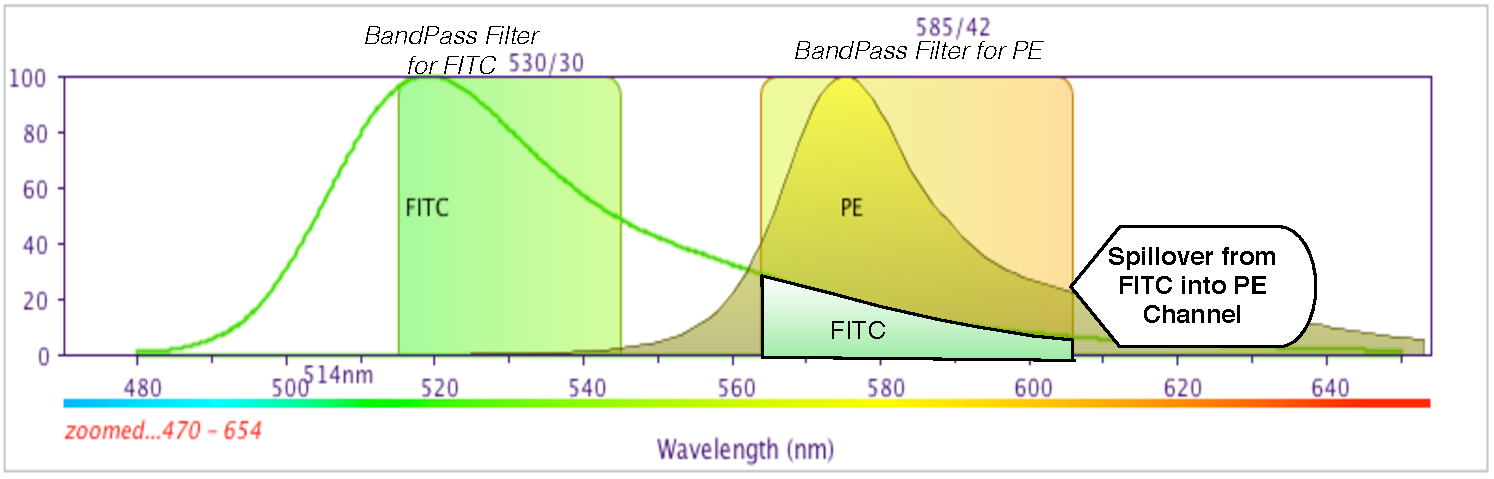
\includegraphics[scale=0.6]{introduction2/figures/spillover.pdf}
\end{center}
\mycaption{figure:spillover}
{ Leaking of signal from FITC fluorochrome into PE detector.}
{
  \small{Created using: \url{http://www.bdbiosciences.com/research/multicolor/spectrum_viewer/}}
}
\end{figure}
The matrix solution is known as the spillover matrix and is usually a square matrix with as many rows as there are fluorochromes and columns as there are detectors.
%if there as many dyes as there are detectors 
To calculate the spillover matrix, single coloured beads are used. 
The pairwise contribution of a fluorochrome to a non-specific channel is then summarised as a compensation matrix (\Cref{table:spillover}).
%To account and correct for this, the overlap needs to be assessed by evaluating the pairwise contribution of the signal of one fluorochrome to that of an other.
%These pairwise values can then be summarised in what is known as a spillover or compensation matrix (Table\ref{table:spillover}).
%This phenomenon is known as spectral spillover.
By subtracting the spillover values from the mixed intensity one can then recover the original intensity.
This compensation step is usually performed after all the data from an experiment has been collected before commencing analysis.  
\begin{table}[h]
\begin{center}
\begin{tabular}{rrrrrrr}
  \hline
%\backslashbox{Signal}{Detector} & Alexa-488 & PE-Cy7 & APC & PE & Alexa-700 & Pacific Blue \\ 
\backslashbox{Signal}{Detector} & PMT 1 & PMT 2 & PMT 3 & PMT 4 & PMT 5 & PMT 6 \\ 
  \hline
Alexa-488    & 100 &   0 &   0 &  16 &   0 &   0 \\
PE-Cy7       &   0 & 100 &   0 &   1 &   2 &   0 \\
APC          &   0 &   0 & 100 &   0 &  30 &   0 \\
PE           &   2 &   1 &   0 & 100 &   0 &   0 \\
Alexa-700    &   0 &   1 &   2 &   0 & 100 &   0 \\
Pacific Blue &   0 &   0 &   0 &   0 &   0 & 100 \\
   \hline
\end{tabular}
\end{center}
\mycaption{table:spillover}
{ Spillover matrix of the fluorochomes used by \citet{Dendrou:2009dv} obtained using single colour beads. }
{
Each entry is the percentage of the emitted fluorochrome signal (row) picked up by a detector (column).
The rows represent the fluorochomes and the columns are the PMT detectors.
Each detector is tuned to capture the intensity of a single fluorochrome (diagonal entries).
Spillover occurs when certain fluorochromes are detectable by more than one detector (non-zero terms off the diagonal).
Notice that there is non-negligeable spillover (\SI{30}{\percent}) of APC into PMT 5, the detector meant for Alexa-700.
}
\end{table}

%\subsection{What is Flow Cytometry, How Does it Work?}
%First the sample is prepared.
%Cells are labelled with various antibodies conjugated with different fluorescent probes which bind to specific targets inside or on the surface of the cell with the aim
%of uniquely labelling different cellular markers.
%The sample is then fed to the flow cytometry instrument.
%The cells in the sample are hydro-dynamically focused so that they file up as they go through one or more lasers.
%The purpose of the lasers is to excite the fluorescent probes attached to the cell which then let off a fluorescent signal whose intensity
%is captured by a number of receptors.
%Different receptors are designed to measure different ranges of intensities.
%The strength of the signal correlates with the number of fluorescent probes which are attached to the target.
%Another type of measure which is captured is how the light from the laser scatters as it hits the cell.
%Side scatter tends to correlate with the density of the cell whereas forward scatter tends to correlate with the size of the cell.
%In practice however many complications can occur during the preparation and running of the sample.
%Cells may clump together, antibodies may be none specific, cells die causing cell debris, fluorochromes can deteriorate and not fluoresce in the expected spectrum.
%All these factors tend to result in erratic or misleading fluorescence reading which contribute to making the results noisy and hard to analyse.

Compensation to account for fluorescence crosstalk, is just one of the intricacies of flow data.
Other intricacies are data format
and the choice of
the data transformation,
%variance-stabilising transform
which can both have an important impact on the analysis.

\paragraph{Flow cytometry data format}
The data format determines the range and the precision of the data stored.
The objective of the \gls{FCS} is to define a unified file format for flow data
that allows files created by one type of acquisition hardware and software to be analyzed by any other type.
The first \gls{FCS} format for data files was FCS 1.0 \citep{Murphy:1984ev}.
The standard was later updated in 1990 as FCS 2.0 \citep{Anon:1990ce} and again in 1997 as FCS 3.0 \citep{Anonymous:vr}.
FCS 2.0 and FCS 3.0 are the current two main competing standards.
FCS 2 is a logarithmically compressed format which does not allow negative intensities.  
Instead negative values reported by the instrument are arbitrarily assigned the minimum value.
This leads to what is described as the log artefact: a pile up of intensities on the axes for low intensity values.
FCS2 data are integers in the range $1$ to $10000$ (4 decades).
FCS 3 on the other hand is closer to the raw data, covers a greater range and allows for negative values.
FCS 3 leaves more flexibility to the choice of transform.
FCS 3 are floating point numbers in the range $-211$ to $262143$ (8 decades)
FCS 2 is more trivial to process as it requires practically no post processing except for a log transform.
FCS 3 requires more careful thought as it leaves to us the compensation and the choice of a suitable transformation.
For low intensity fluorescence, FCS 3 is the preferred format as the truncation at zero of intensity values for FCS 2 can lead
to loss of information (\Cref{figure:fcs2-fcs3}).
%In my work so far I have been using FCS 2 to facilitate comparison to the manual analysis but in the future I intend to use FCS 3 instead.  
%FCS 2 has compensation pre-applied whereas in FCS 3 compensation matrix is stored as part of the data format and needs to be applied manually.
%Unfortunately due to limitations of the fluorescent dyes and the instrument, the fluorescent signal measured in on channel is often a mixture of signals.
%This phenomenon is known as spectral spillover.
%The deconvolution of this signal is a process known as compensation.  The matrix solution is known as the spillover matrix
%and is usually a square matrix if there as many dyes as there are detectors.
\begin{figure}[h]
\centering
\begin{subfigure}[b]{.4\textwidth}
    \centering
    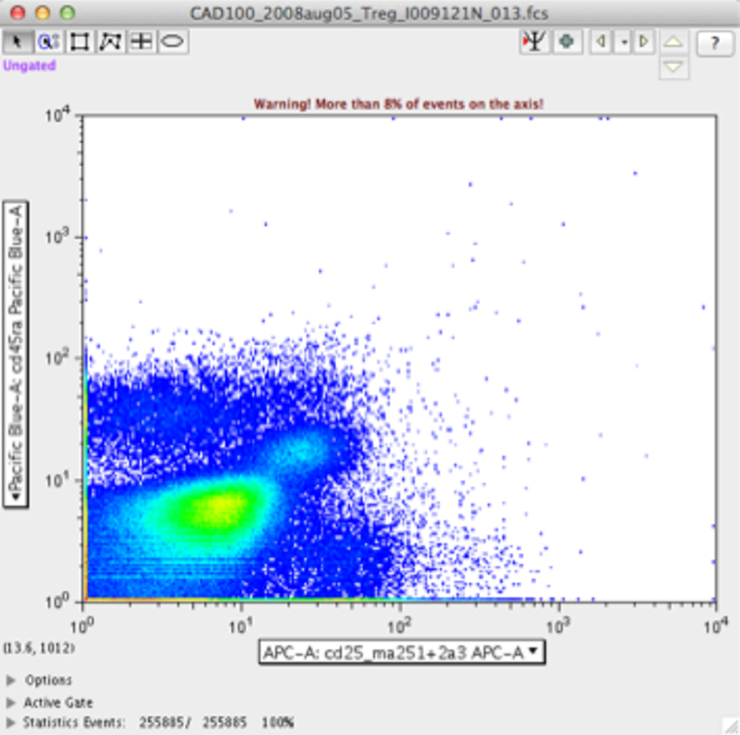
\includegraphics[scale=.3]{figures/fcs2.pdf}
    \caption{ FCS 2 }
\end{subfigure}
~
\begin{subfigure}[b]{.4\textwidth}
    \centering
    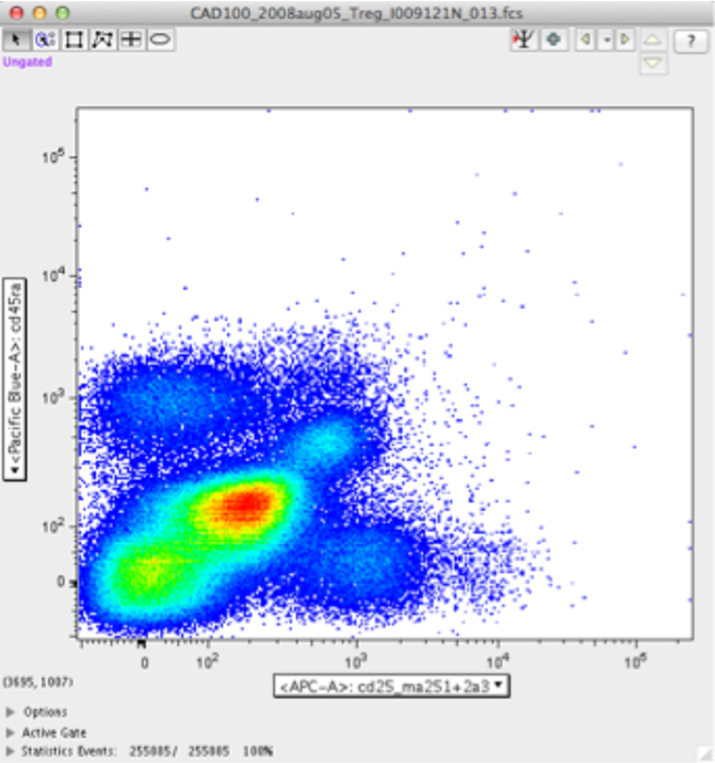
\includegraphics[scale=.3]{figures/fcs3.pdf}
    \caption{ FCS 3 }
\end{subfigure} 
\mycaption{figure:fcs2-fcs3}
  {The same data encoded in FCS2 (a) and FCS3 (b).}
  {
    %FCS 2 truncates intensity values at zero while FCS 3 allows for negative intensities.
    In FCS 2 (a), truncation at zero leads to loss of low intensity clusters as compared to FCS 3 (b).
  }
\end{figure}


\paragraph{Data transformation for display and analysis}
%FCS data needs to be rescaled for Display and Analysis}
As fluorescence intensity tends to scale multiplicatively, intensity data needs to be linearised for the purpose of visualisation and clustering.
Clustering algorithms based on variance (average distance to the mean) perform poorly on skewed data, and in general humans are more comfortable dealing
with data on a linear scale.
%Given a finite range (number of channels/bins), a logarithmic transform can be used to maximise the range of data that can be captured by a detector.
Given FCS 2 data is strictly positive, a simple $\log_{10}$ transform is usually applied to linearise the data.
As FCS 3 allows for negative values a different transform is required.
Transforms which are closer to linear near zero are preferred, 
since the logarithmic transform is distorting (\Cref{figure:log10-deform})
for low intensity values \citep{Durbin:2002tj,Tung:2006uw}.
\begin{figure}
\centering
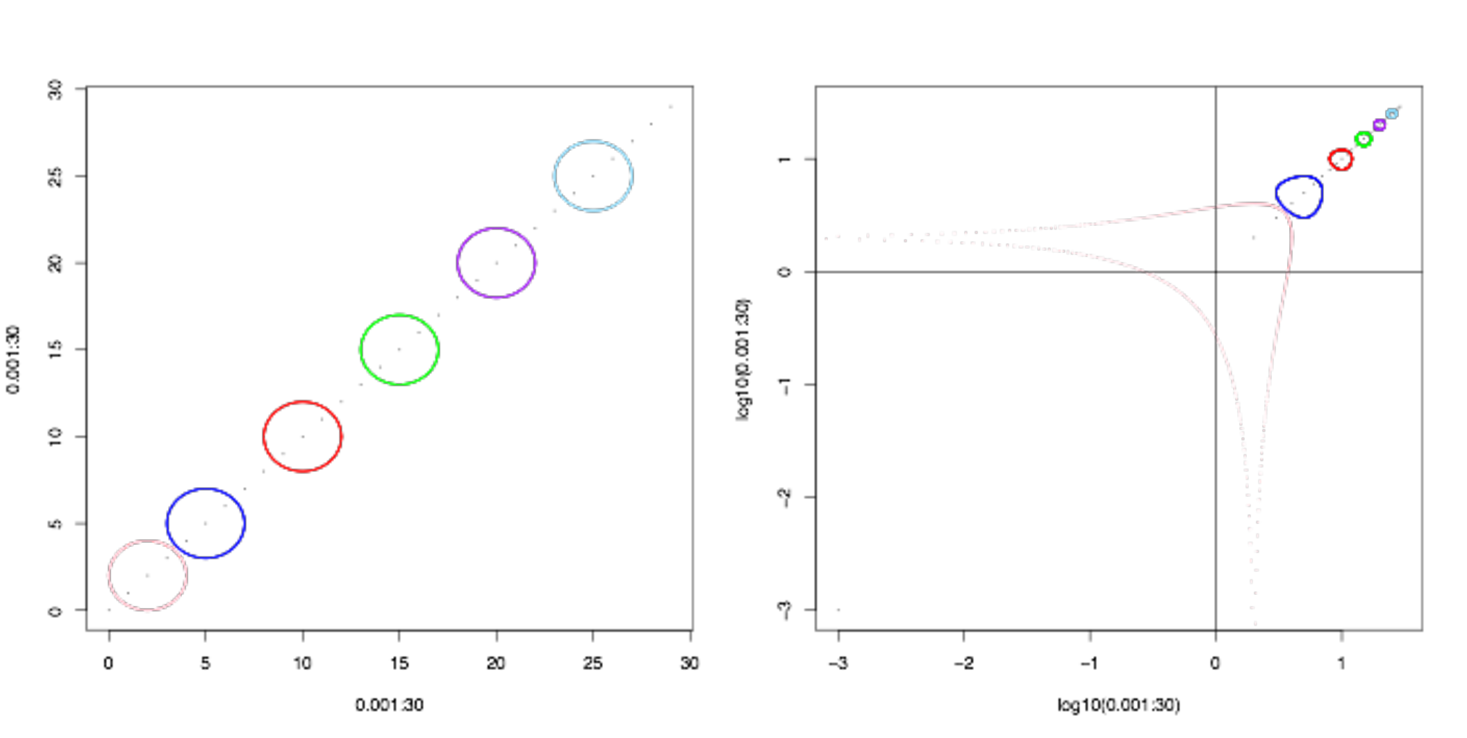
\includegraphics[scale=.5] {Appendix/figures/log10-deform.pdf}
\mycaption{figure:log10-deform} 
{Log transform inflates the variance around zero.}
{
  Depicted on the left are circles of equal diameter viewed on a linear scale.
  These circles represent spherical two-dimensional Gaussian distributions, 
  When a logarithm transform is applied, the shape of the circles are distorted and they no longer have the same area.
  Close to zero, the area of the circles increases and their shape is distorted.
  This would translate into an increase of the covariance for a Gaussian distribution.
}
\end{figure}
%this transform distorts the data: it shrinks the distance between points making clusters less distinguishable
Some appropriate transformations for FCS 3 are the Generalized Arcsinh, the Logicle transform,
the LinLog and the Generalized BoxCox \citep{Bagwell:2005he,Parks:2006gaa,Finak:2010is}.
Given the data, parameters for these transformations can be estimated using maximum likelihood assuming a multivariate Gaussian distribution of the data \citep{Finak:2010is}. 
However as illustrated by \citet{Tung:2006uw}, care needs to be taken as the transforms can introduce spurious peaks in the intensity distribution around zero.
The Logicle transform as defined by \citet{Parks:2006gaa},
is the most widely used transform for FCS 3 data and is the one I will be using in this thesis.
It takes as input the w parameter which influences the linearization width around zero in asymptotic decades.
The influence of the w parameter on the shape of the transformed intensity distribution is illustrated in \Cref{figure:logicle-transform-w}.
%\Cref{figure:logicle-transform}.
%w parameter should be greater 0 and 
%and does not exist in closed form but instead is estimated numerically from its inverse which is the Biexponential transform:
%\[
%T*10**-(m-w-a) * (10**(x-w-a) - p**2 * 10**-((x-w-a)/p) + p**2 - 1)
  %f^{-1}(x;\theta) = a e^(b(x-w)) - c e^(-d(x-w)) + f
%\]
%# @param w is the linearization width in asymptotic decades. w should be > 0 and determines the slope of transformation at zero.
%# w can be estimated using the equation w=(m-log10(t/abs(r)))/2, where r is the most negative value to be included in the display
%# @param t	Top of the scale data value, e.g, 10000 for common 4 decade data or 262144 for a 18 bit data range. t should be greater than zero
%# @param m is the full width of the transformed display in asymptotic decades. m should be greater than zero
%# @param a	Additional negative range to be included in the display in asymptotic decades. Positive values of the argument brings additional negative input values into the transformed display viewing area. Default value is zero corresponding to a Standard logicle function.
%assume a global distance metric.
%as illustrated in Figure~\ref{figure:transform}.
% Another possibility is the arcsinh transform which allows for negative values without requiring an offset to be specified:
%\[
    %f(x) = \operatorname{arcsinh}(x) = \log( x^2 + \sqrt { 1+ x^2 } )
%\]
%Update for the Logicle Data Scale Including Operational Code Implementations \citet{Moore:2012gz}
\begin{figure}[h]
\centering
\begin{subfigure}[b]{.4\textwidth}
    \centering
    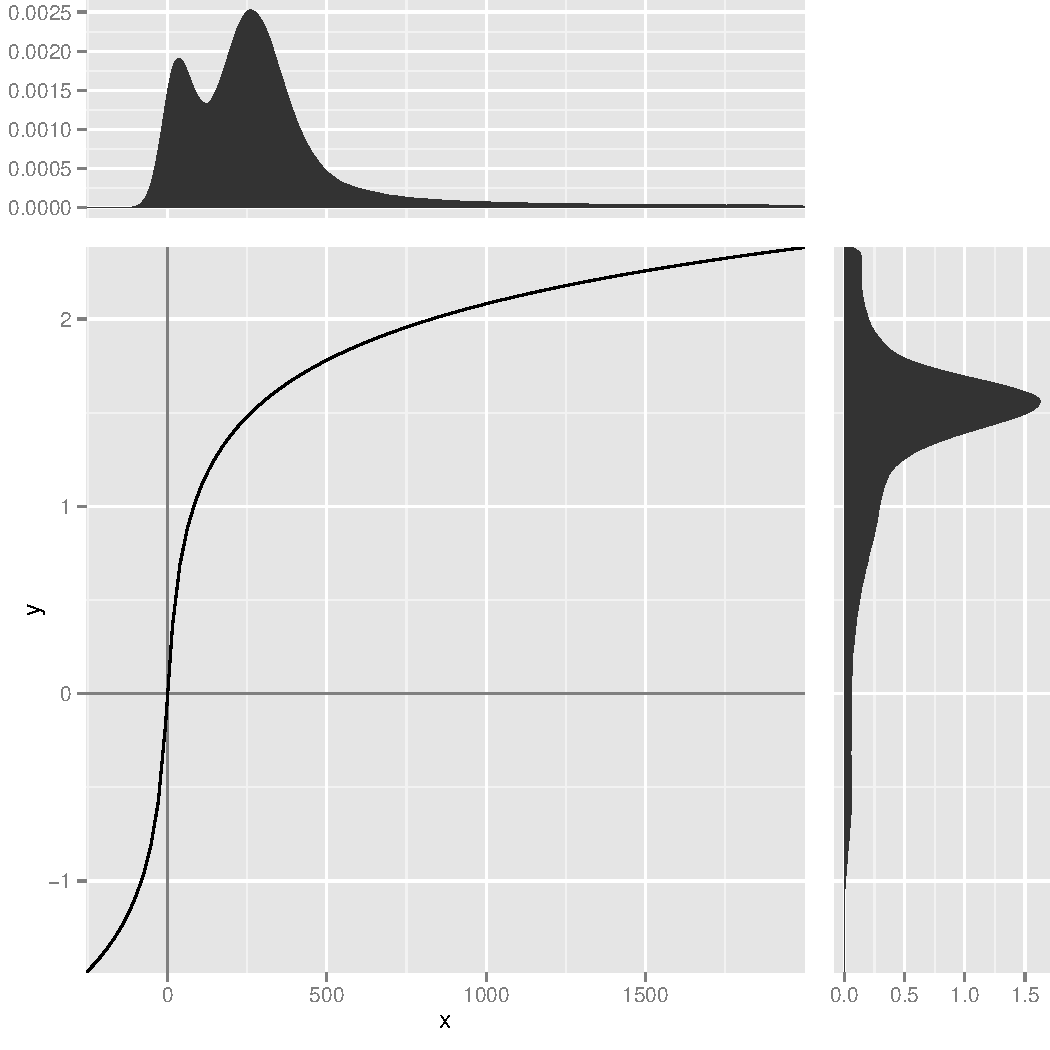
\includegraphics[scale=.3]{Appendix/figures/logicle-transform-a.pdf}
    \caption{w=0}
\end{subfigure}
~
\begin{subfigure}[b]{.4\textwidth}
    \centering
    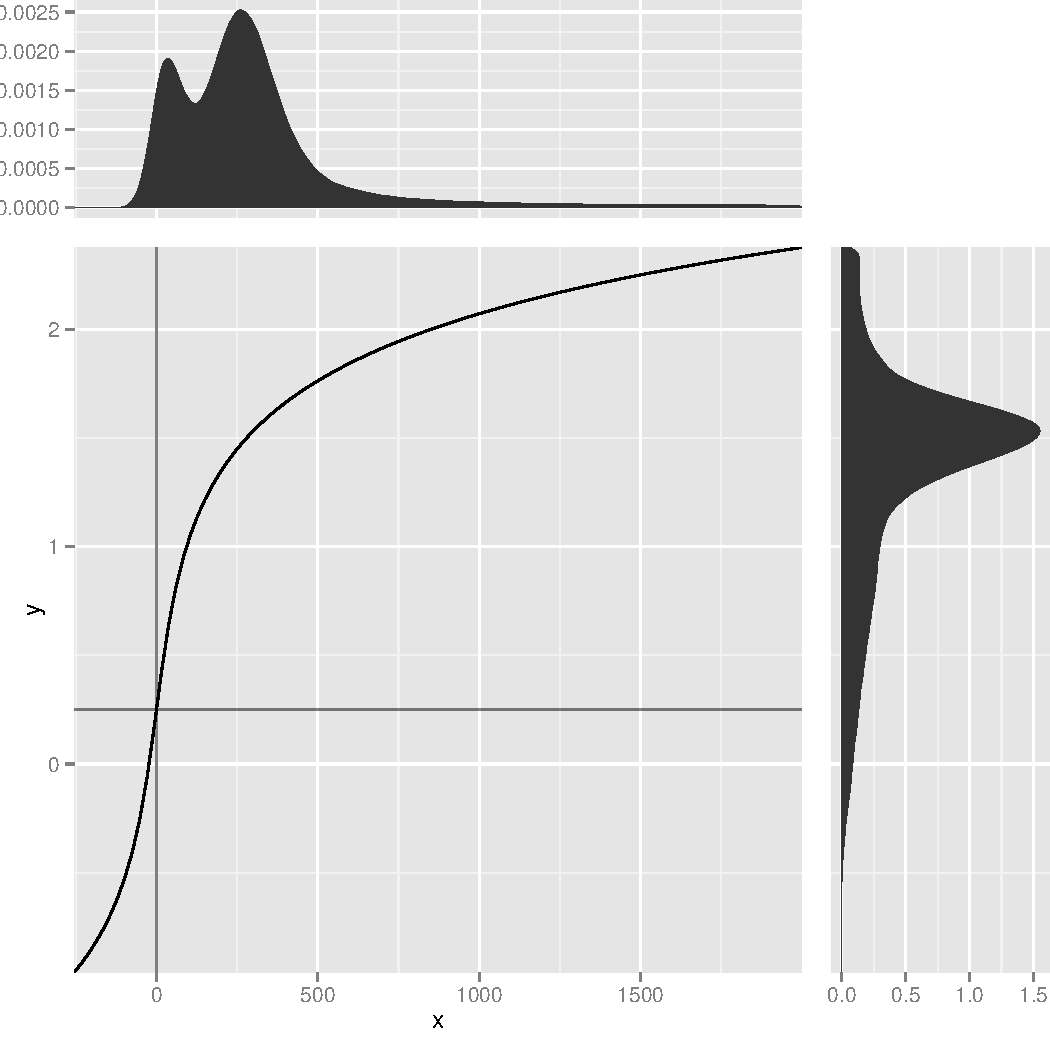
\includegraphics[scale=.3]{Appendix/figures/logicle-transform-b.pdf}
    \caption{w=.25}
\end{subfigure}
~
\begin{subfigure}[b]{.4\textwidth}
    \centering
    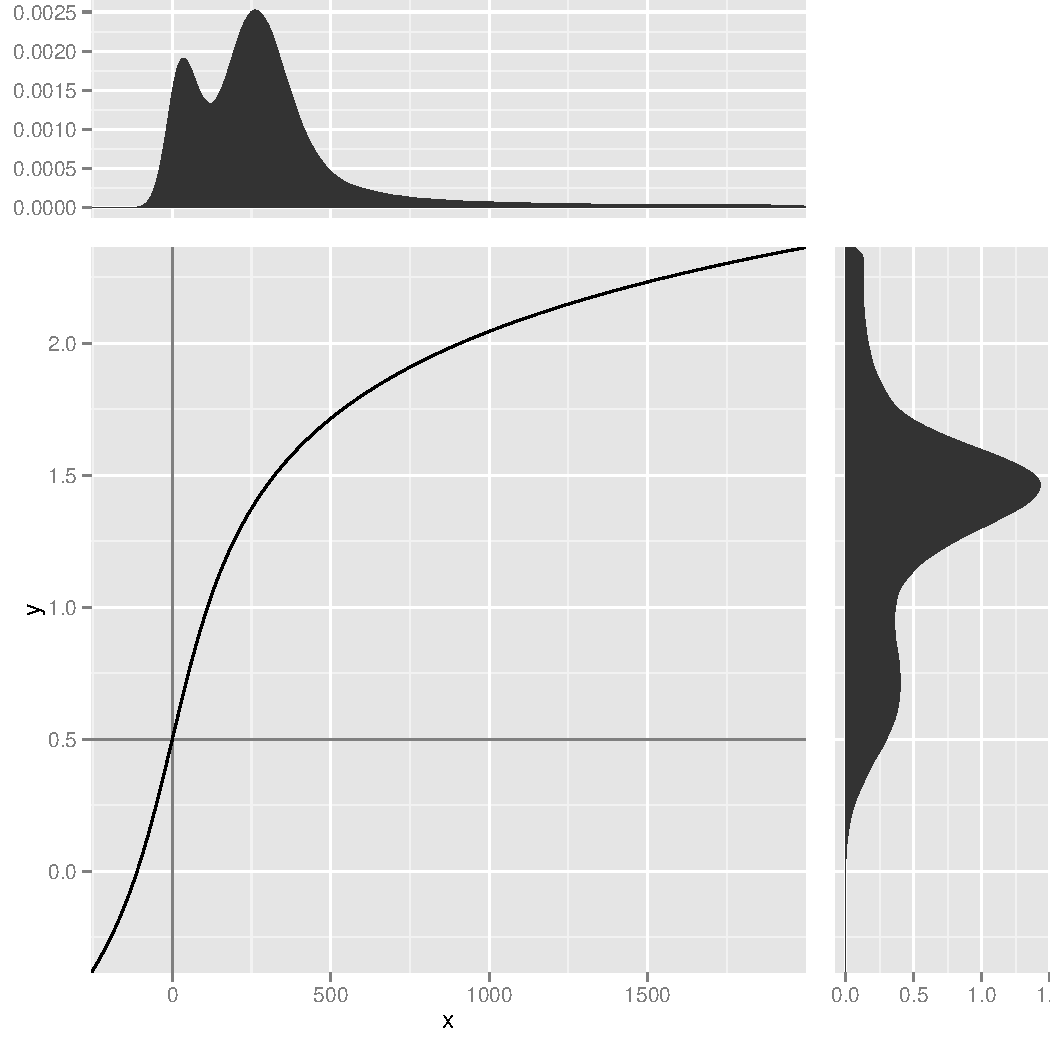
\includegraphics[scale=.3]{Appendix/figures/logicle-transform-c.pdf}
    \caption{w=.5}
\end{subfigure}
~
\begin{subfigure}[b]{.4\textwidth}
    \centering
    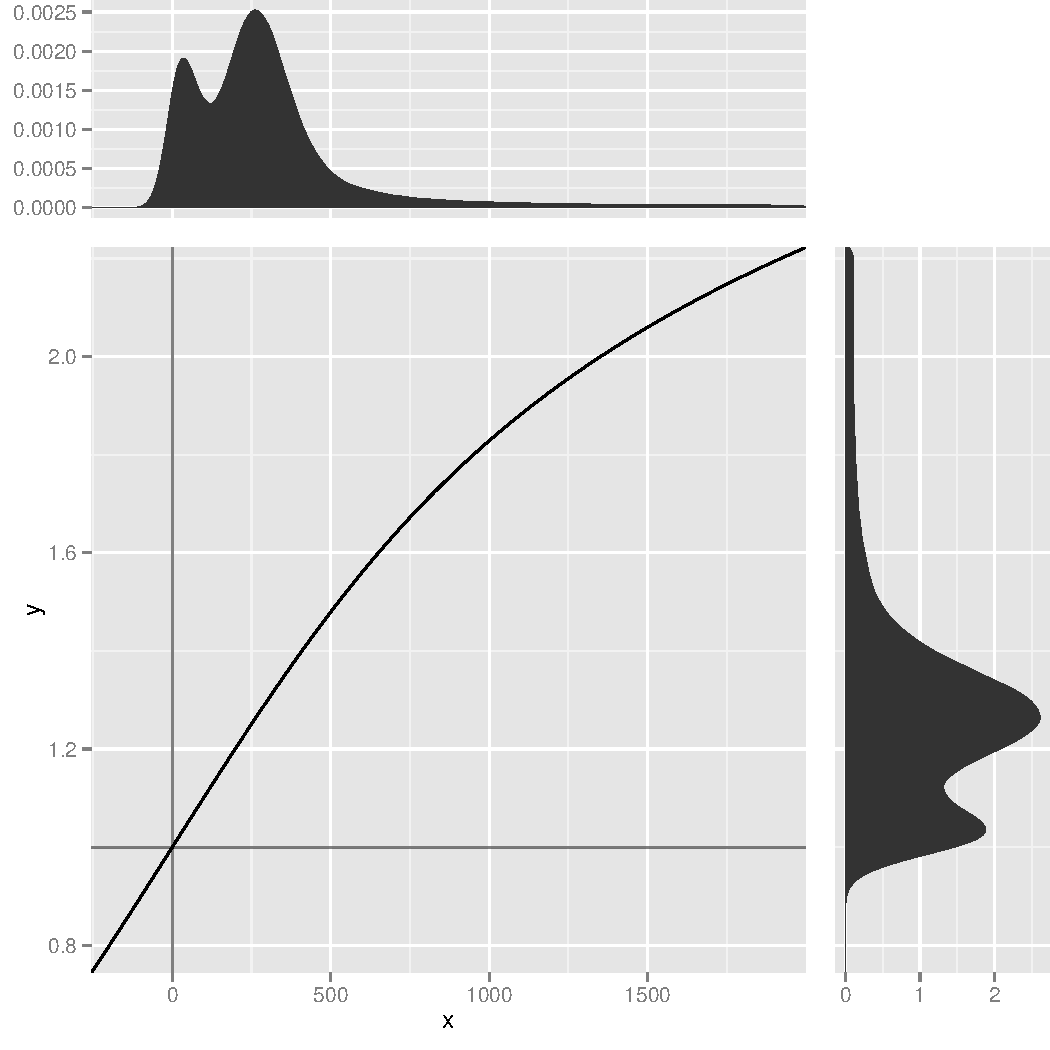
\includegraphics[scale=.3]{Appendix/figures/logicle-transform-d.pdf}
    \caption{w=1}
\end{subfigure}
\mycaption{figure:logicle-transform-w}
{Effect of different values of w parameter of the Logicle transformation on the data distribution.}
{
  The Logicle transform maps the data distribution defined on x to the data distribution defined on y.
  The transform approximates a linear transform near zero and a log transform elsewhere.
  The w parameter maps the zero of the transform to w.
}
\end{figure} 
%\begin{figure}[h]
%\centering
%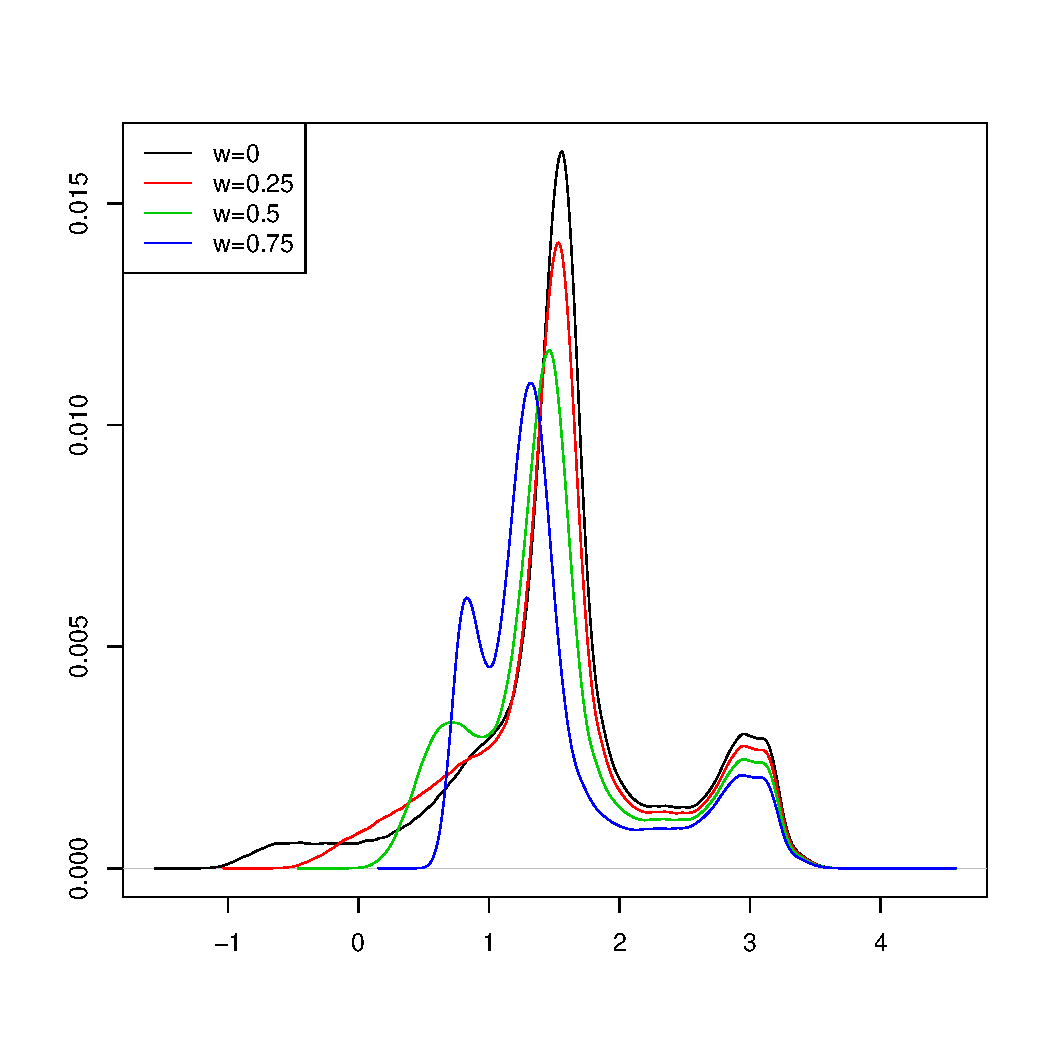
\includegraphics[scale=.5] {Appendix/figures/logicle-transform.pdf}
%\mycaption{figure:logicle-transform} 
%{Logicle transformed data}
%{
  %The Logicle transform approximates a linear transform around the first decade
  %and a log transform elsewhere.
  %similar to a logistic function ?
  %As the w parameter increases from 0 to 0.75 the is squashed
  %As the slope of the linear transform, increases the shape of the distribution approximates the shifted log transform in \Cref{figure:log10-transform}.
%}
%\end{figure}

% NOTE: The shifted log transform is silly because values within -100;100 should probably not be log transformed.

%For the purpose of gating the bead data, the transform chosen for FCS2.0 data is a standard log transform (offset $b=0$)
%whereas for FCS3.0 we use an offset $b=50$ so to make all values positive:
%\[
    %f(x) = log(x+50)

%One issue in choosing a transform is whether to allow for negative values.
%The simplest transform which can cater for negative values is a log transform with an offset parameter:
%\[
    %f(x) = \log_{10}(x+b)
%\]
%However this is not ideal as it merely creates an (\Cref{figure:log10-transform})
%In fact simply ignoring the zero values would be more appropriate
%\begin{figure}[h]
%\centering
%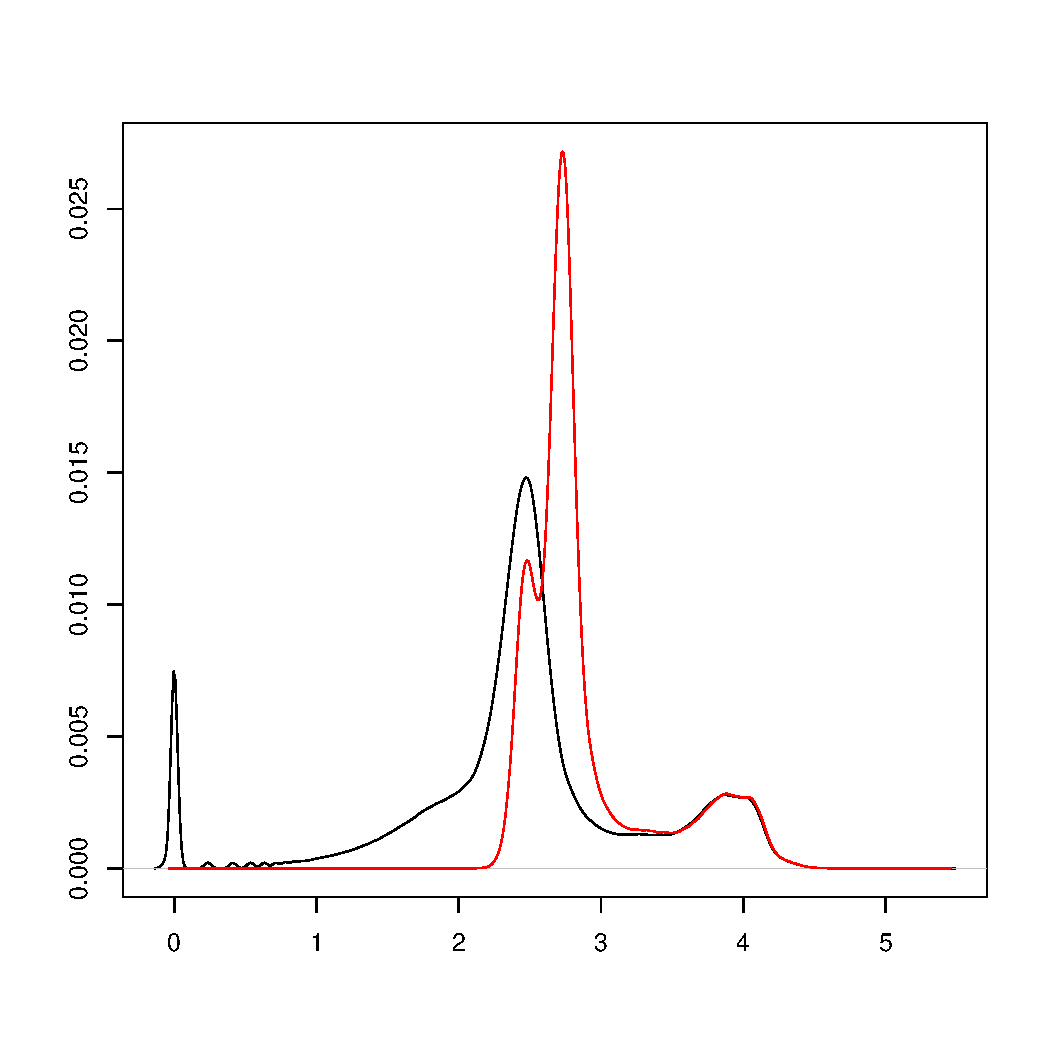
\includegraphics[scale=.5] {Appendix/figures/log10-transform.pdf}
%\mycaption{figure:log10-transform} 
%{$Log_{10}$ transformation on FCS 3 data}
%{
  %In black, the transform assigns intensity values of zero or less to zero.
  %In red, all the intensity values have been shifted by the minimum, before applying the transform, so that all negative values are greater than zero.
  %In this scenario, this is not ideal as it introduces a spurious peak.
  %Mapping to zero or simply discarding negative intensity values would be a more sensible approach here.
%}
%\end{figure}


\clearpage


\paragraph{Noise in flow cytometry} 
Beside these data format and transformation intricacies, there are many sources of noise in flow cytometry which complicate sample comparison and impact reproducibility.  
\begin{itemize}
  \item \textbf{Sample processing and storage conditions noise.}
    Certain surface markers are more fragile than others and may be shed when cells are frozen for storage.
    Also certain chemical treatments like permeabilisation can affect the quality of the staining.
    %Depending on the day of analysis, samples might look remarkably different.
    %For this reason it is preferable to analyse multiple samples on the same day where possible.
  \item \textbf{Noise associated with the staining of the sample.}
    The qualitative and quantitative choices for selecting antibodies and fluorochromes influence the quality of the staining.
    Antibodies have a tendency to be sticky and can bind to other targets in an erratic manner leading to spurious signal.
    The level of non-specific binding can be assessed with isotype antibodies.  
  \item \textbf{Noise linked to the instrument.}
    The reliability of the lasers and detectors may wither with time.
    Fluorescent beads can be used to detect and correct these variations.  
  \item \textbf{Noise due to the flow operator.}
    Sometimes the operator might decide to not collect all the events and for example apply a cutoff on the side and forward scatter.
\end{itemize}
All these sources of noise contribute to different patterns of staining and concentrations of debris
which may lead to spurious cell populations or skew the analysis, complicating the analysis across samples and laboratories.
Some of these issues are being addressed by the \gls{HIP} consortium standardisation efforts \citep{Maecker:2012gl}
which aims to enhance reproducibility of flow analysis results across laboratories,
through the use of lyoplates, and agreement on experimental protocols and instrument configurations.
However data analysis techniques such as normalisation are still necessary to deal with residual noise.

\section{Normalisation}
%\section{Normalisation: why it is needed, methods, utility}

%Heraclitus said `` you cannot step into the same river twice ''
%Experiments in biology are very difficult to replicate exactly for technical and biological reasons.
The purpose of normalisation is to remove unwanted experimental variation to make data comparable even when the samples are
collected on different days, processed with different protocols or instrumental configurations.
%The underlying principle being that true biological variation is specific whereas experimental variation affects the whole sample.
Nonetheless, distinguishing between unwanted and biological variation necessitates some prior knowledge about the datasets,
either in the form of global distributional assumptions or in the form of local features which exist in a predictable relationship across samples.
In microarray gene expression datasets, for example, one distributional assumption is that the majority of genes are not differentially expressed between similar samples,
hence the expected log ratio of gene expression in two samples should be centered on zero \citep{Smyth:2003ie,Bolstad:2003ia}.  
It is also possible to use reference points to normalise across samples
%decouple technical variation from biological variation
%without making global distributional assumptions,
by using local features of the distribution or objects with known properties, such as beads in flow cytometry or reference probes in microarrays.
%These features can also be added to the sample, commonly known as spike-ins, or
In microarray, since the number of data points is constant and the distributions are unimodal across samples,
normalisation methods like quantile normalisation perform well \citep{Bolstad:2003ia}.
However in flow cytometry, this type of normalisation is not appropriate because samples contain different number of events and 
the distributions are typically multimodal, as commonly found in datasets containing mixtures of groups.
%The modes of the distributions or peaks of the density function, represent the average protein quantity carried on the surface of different cell types.
While in theory, the locations of these modes or peaks of the density function should remain fairly stable across samples provided experimental parameters are kept constant,
in practise there is often variation attributed to factors which are beyond our control such as long-term instrument decalibration.
On the other hand, the height of the peaks, the relative frequencies of the cell populations, are expected to change since they are
are sensitive to sampling variation.
%In the case of qPCR data, the groups are representative of the copy numbers.
%and cells cannot be matched across samples in the way microarray probes are.  
%If the features are modes in the data, then normalisation is equivalent to doing clustering, in order to identify modes, followed by meta-clustering to match the modes across samples.
%While these methods have been successfully applied to microarray data, they are not generally applicable to multimodal univariate distributions commonly found in datasets containing mixtures of groups.
These observations motivate a normalisation method which aligns the peaks of the distributions so that cell populations are centered
in a similar location across samples even when their relative proportions changes.
The implementation of this normalisation method then depends on the technique used to identify and match the peaks across samples.
%The ideal scenario is when the number of peaks is known and constant across samples.
%More flexible peak searching algorithms are required to allow for this per sample-variation.
One method of identifying peaks of the density function is with a sliding window approach.
The sliding window records the point with the highest density estimate in the current window and
returns a list of highest density points of which the top K may be chosen.
This is one of the approaches implemented in the \BioConductor{flowStats}.
\Cref{figure:normalisation-peaks} illustrates this method on real flow data where two common groups stand out and are reasonably well separated.
Unfortunately, peaks are not always consistently identifiable across samples.
In these cases, it may be preferable to only identify the most distinguishable subset of peaks, those representative of the most common groups,
in order to do the alignment.
%This is the case when dealing with synthetic data such as beads.
%In this scenario, basic clustering algorithms as covered in the next section, can be applied to identify the peaks in each sample.
%This is the method which I have developed in the \Rpackage{flowBeads} BioConductor package which identifies bead populations with the K-medoids algorithm
%for the purpose of fluorescence normalisation.
%This is the method I applied in the qPCR data, in \Cref{chapter:kir}, to align common copy number groups 1 and 2 across plates.
%However peaks are not always easily identifiable.
%% Peaks
\begin{figure}[h]
\begin{subfigure}[b]{.5\textwidth}
\centering
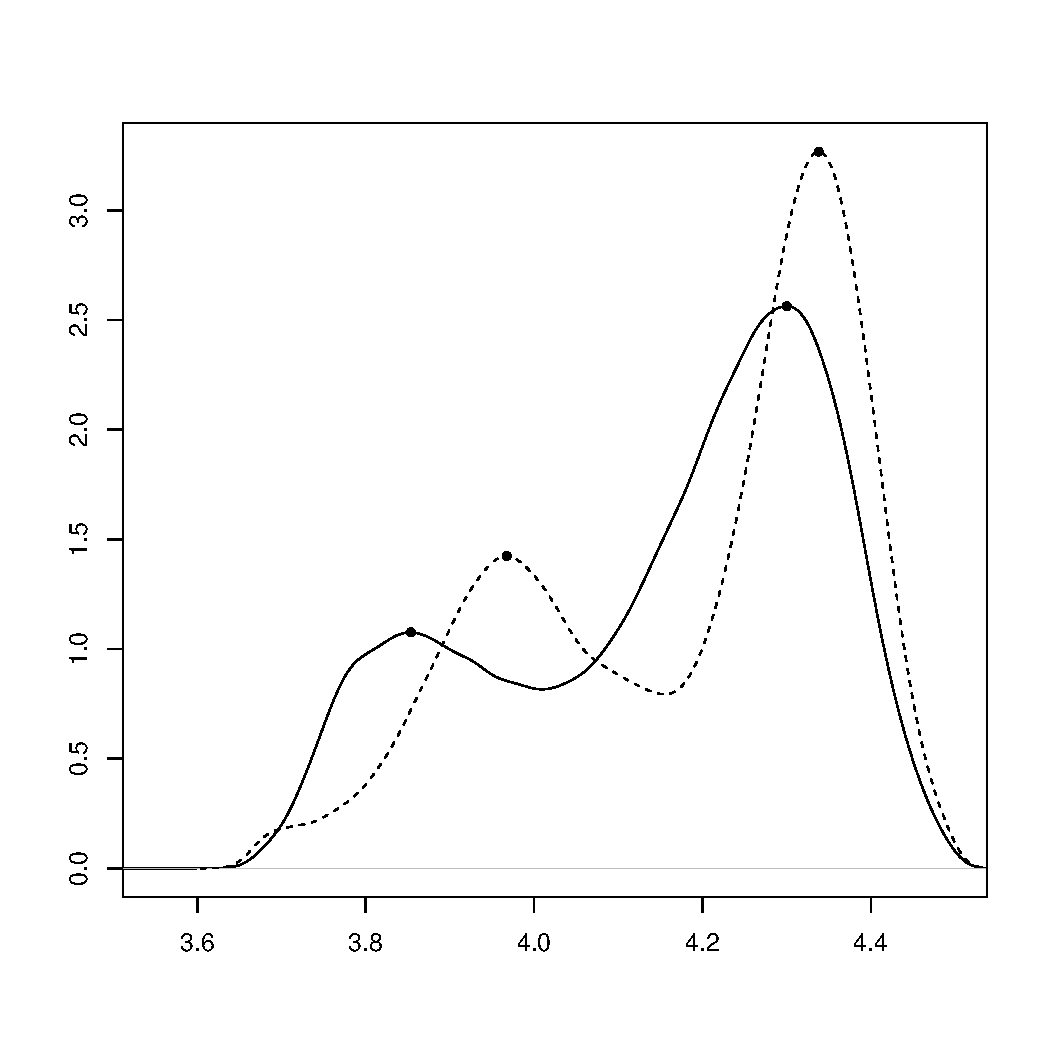
\includegraphics[scale=.4]{figures/normalisation-peaks-a.pdf} 
\caption{identification of peaks}
\end{subfigure}
~
\begin{subfigure}[b]{.5\textwidth}
\centering
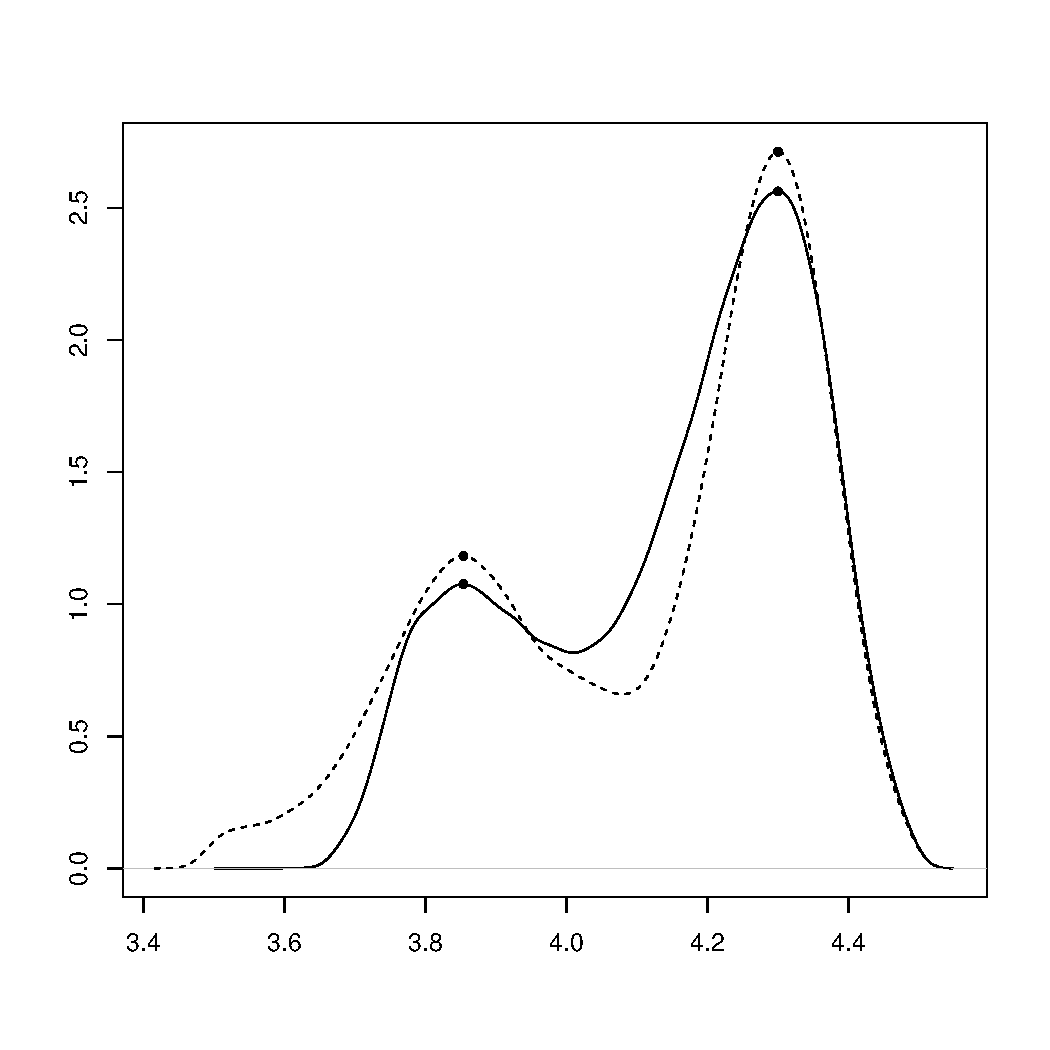
\includegraphics[scale=.4]{figures/normalisation-peaks-b.pdf} 
\caption{peak alignment}
\end{subfigure}
\mycaption{figure:normalisation-peaks}
{Normalisation by peak alignment.}
{
  Distributions of the same marker in two different flow cytometry samples.
  The two peaks of each distribution are identified in (a) using a sliding window of size $40$ on the density function and aligned in (b) using a linear transform.
}
\end{figure}



%In scaling, we subtract the mean and divide by the standard deviation so that the resulting distribution has a mean of zero and a standard deviation of one.
%This approach is sensible if the distibutions are symmetric unimodal like the normal distribution.
%\Cref{normalisation-scaled} is a trivial example of scaling on simulated data.
%$x_0 \sim N
%% Scaling
%\begin{figure}[h]
%\begin{subfigure}[b]{.5\textwidth}
%\centering
%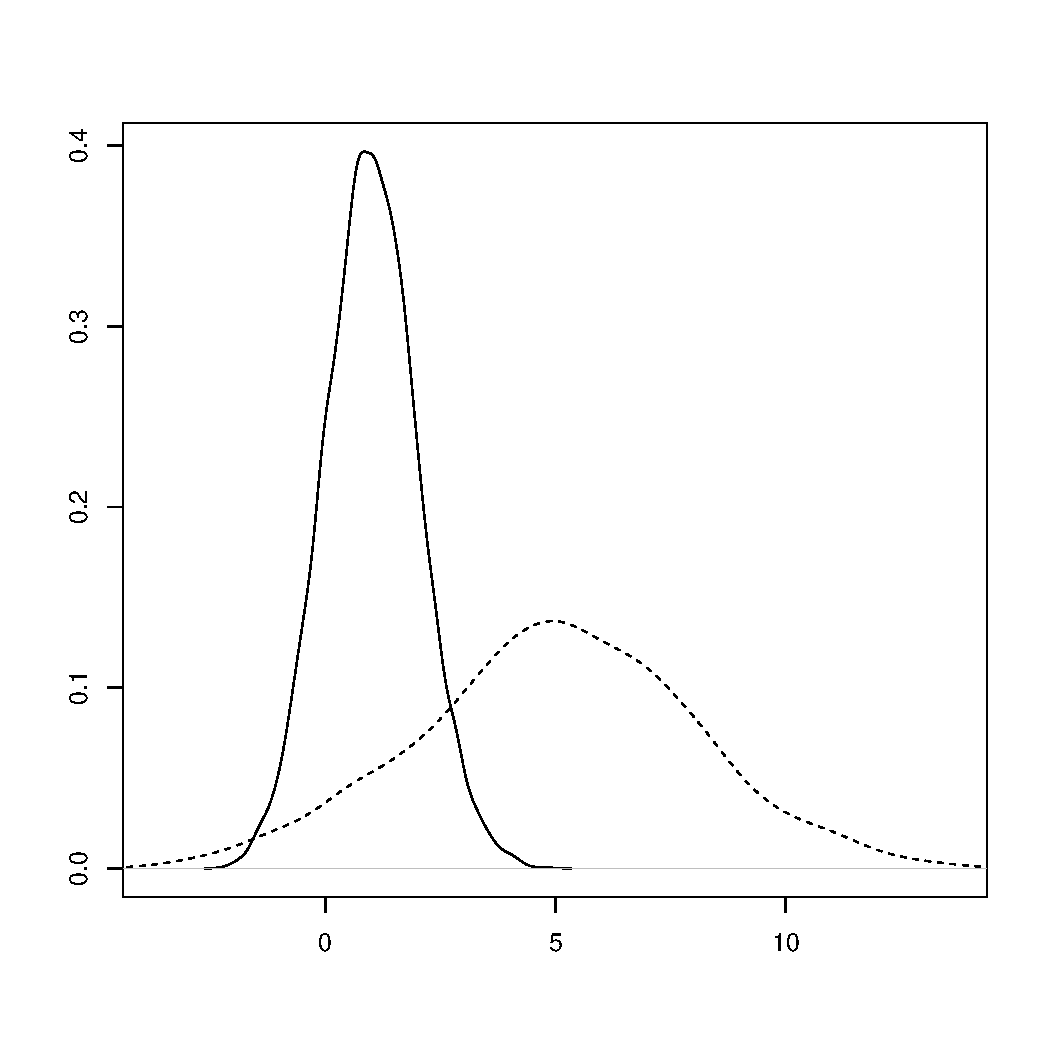
\includegraphics[scale=.4]{figures/normalisation-scaled-a.pdf} 
%\caption{before scaling}
%\end{subfigure}
%~
%\begin{subfigure}[b]{.5\textwidth}
%\centering
%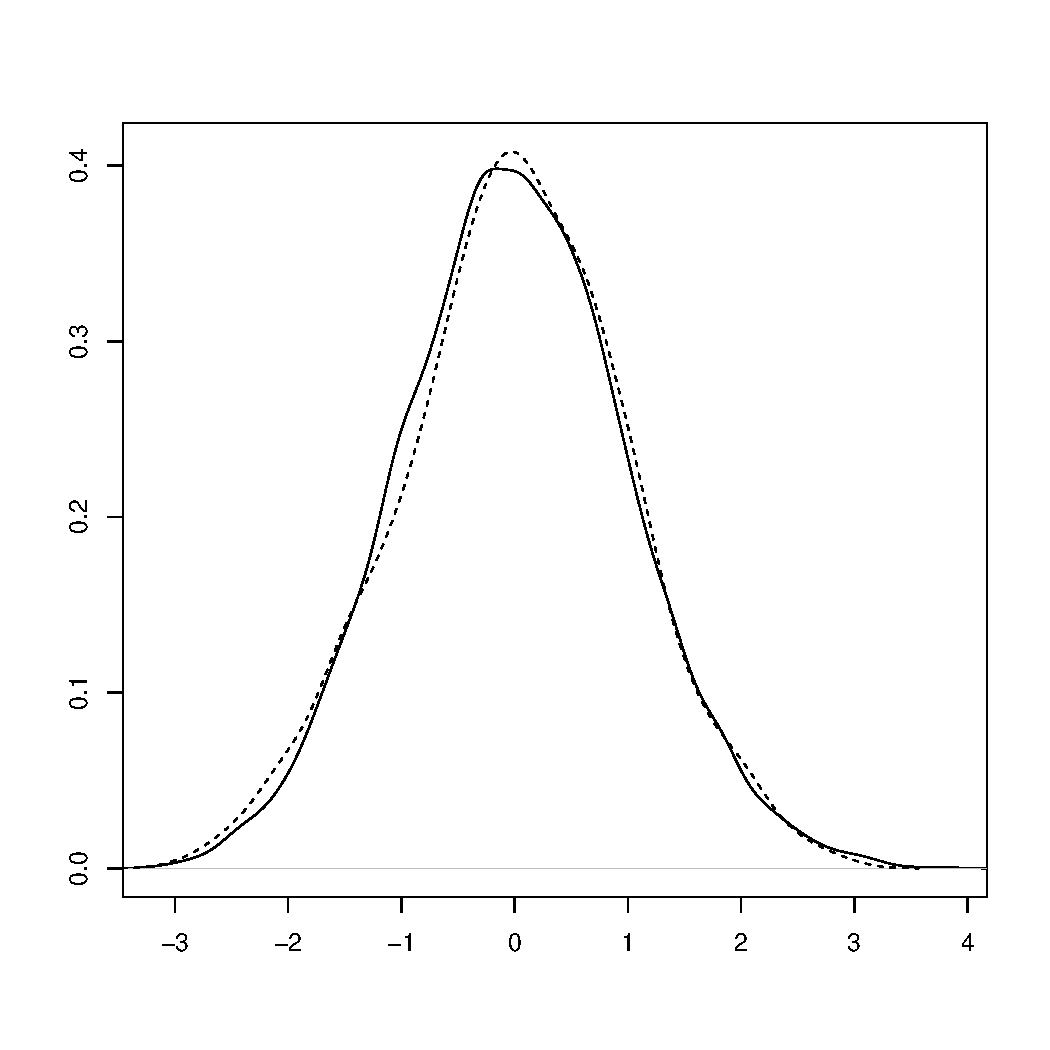
\includegraphics[scale=.4]{figures/normalisation-scaled-b.pdf} 
%\caption{after scaling}
%\end{subfigure}
%\mycaption{normalisation-scaled}
%{Normalisation by scaling on simulated data.}
%{
%In solid black line represents the density function obtained from $10,000$ draws from a normal distribution
%with with means $\mu_0=1$ and standard deviation $\sigma_0=1$.
%The dashed line represents the density function obtained from $1,000$ draws from a normal distribution
%where $\mu_1=5$ and $\sigma_1=3$.
%After scaling both distributions have a mean of zero and standard deviation of one.
%}
%\end{figure}
%If the distributions are unimodal but not symmetric, such as $\chi^2$ distributions, then an alternative is quantile normalisation.
%%As can be seen in \Cref{figure:normalisation-quantile}, the quantiles of the distribution are identified
%%then a transform is applied so that quantiles of one distribution are aligned with those of the other.
%%Here the transform is a simple linear regression.
%%Quantile normalisation works well when the shape of the distributions is the same and only shifted.  
%%% Quantile
%\begin{figure}[h]
%\begin{subfigure}[b]{.5\textwidth}
%\centering
%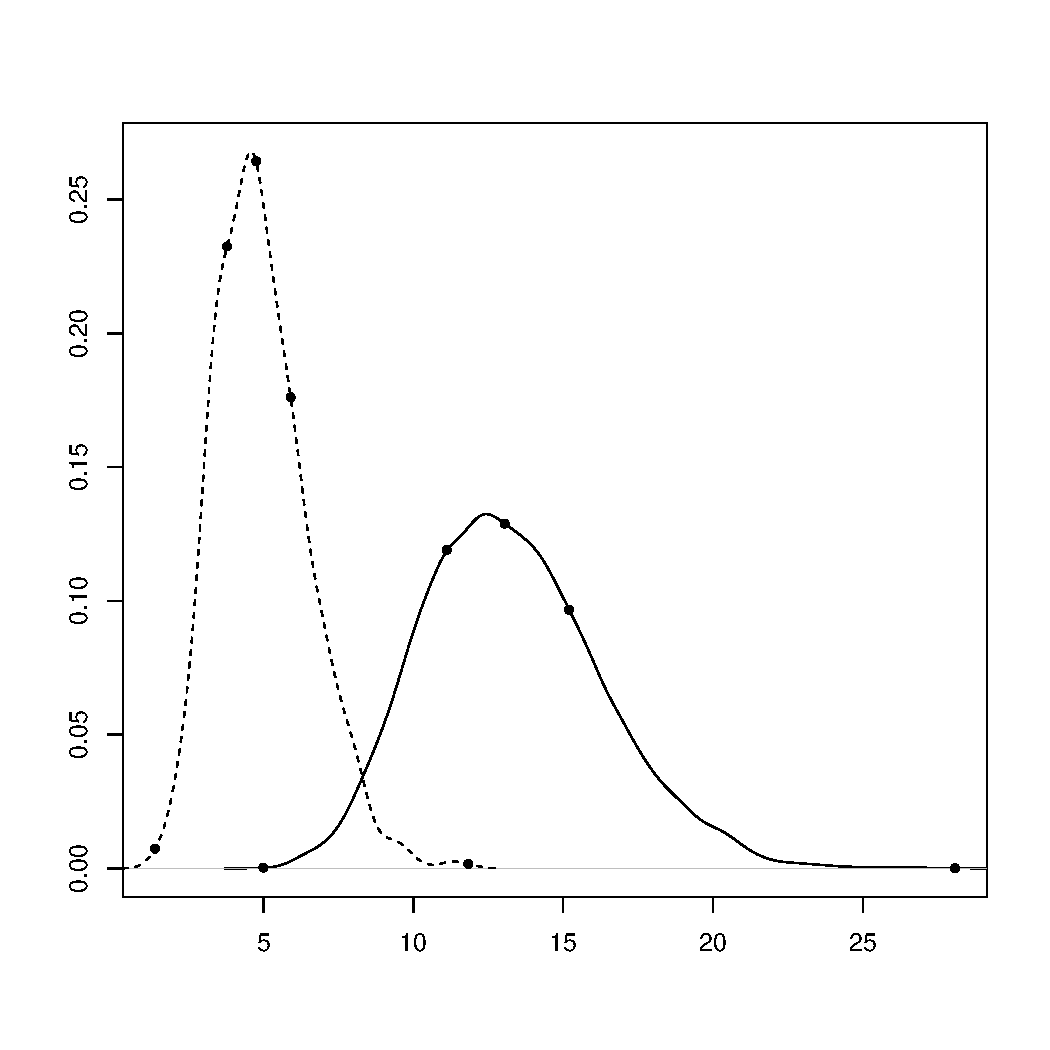
\includegraphics[scale=.4]{figures/normalisation-quantile-a.pdf} 
%\caption{before aligning quantiles}
%\end{subfigure}
%~
%\begin{subfigure}[b]{.5\textwidth}
%\centering
%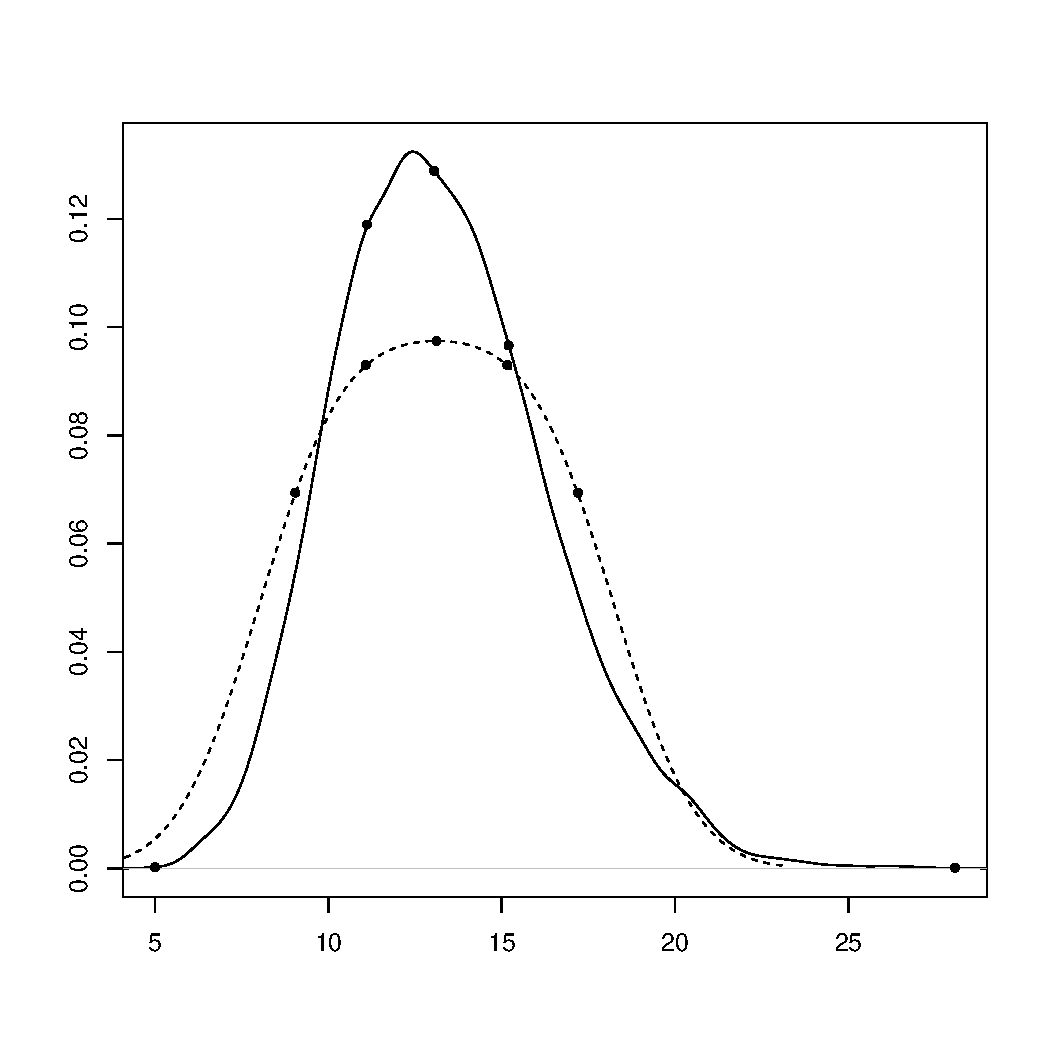
\includegraphics[scale=.4]{figures/normalisation-quantile-b.pdf} 
%\caption{after aligning quantiles}
%\end{subfigure}
%\mycaption{figure:normalisation-quantile}
%{Normalisation by quantile alignment on simulated data.}
%{
%In solid black line represents the density function obtained from $10,000$ draws from a gamma distribution
%with with shape $\alpha_0=20$ and rate $\beta_0=1.5$.
%The dashed line represents the density function obtained from $1,000$ draws from a gamma distribution
%where $\alpha_1=10$ and $\beta_1=2$.
%The black dots are the quantiles.
%The normalisation finds a linear mapping of the quantiles of the dashed-line distribution onto those of the solid-line distribution.
%}
%\end{figure}
%
%Also the M and A should follow the same relationship.  Smoothing methods like loess can also correct MA trends \citet{Smyth:2003ie}.
%But in practise, in brighter spots the balance between the green signal is stronger than the red while in dimmer spots the red signal is stronger than the green.
%This artefact means that low and high intensity genes would wrongly be identified as differentially expressed.
%splines and running median line
%Other methods are quantile or rank normalisation.
%spikeins would be equivalent of inserting beads or the other know entities into our sample
%which can then be used as an internal control.
%MA norm works on 2 dimensions and the probes are known and can be matched across arrays.
%in flow, common cell types are expected to exist across arrays but ungated data does not necessarily match
%because of differences in staining and preparation which creates debris


%\paragraph{Instrument variation}
%\section{Clustering}

%\subsection{Analysis of Results: Identifying Cell Populations and Defining Cell Phenotypes}
%\subsection{Analysis of Flow Data: Identifying Cell Populations}

%Once the data is normalised, we can pool across samples to proceed with cluster analysis, the purpose of which is to identify homogeneous (sharing the same properties) groups (clusters) in the data.
%%TODO normalisation does not usually precede clustering in flow cytometry
%, either pooling the samples together or by clustering them separately.

%The task is to define groups in such a way that data points in the same group are more similar, in some sense or another, to each other than to those in other groups (clusters).

%Clustering is the main task of exploratory and statistical data analysis, used in many fields, including machine learning, pattern recognition, image analysis, information retrieval, and bioinformatics.
%Clustering itself is not one specific algorithm, but the general task to be solved.
%It can be achieved by various algorithms that differ significantly in their notion of what constitutes a cluster and how to efficiently find them.
%Popular notions of clusters are:
%\begin{itemize}
  %\item groups with small distances among the cluster members
  %\item dense areas of the data space
  %\item mixtures of particular statistical distributions
%\end{itemize}
%The appropriate clustering algorithm and parameter settings (including values such as the distance function to use, a density threshold or the number of expected clusters)
%depend on the individual data set and intended use of the results.
%

%\paragraph{Identifying Cell Populations with Manual Gating}
\section{Manual clustering}

Once the data has been made comparable thanks to normalisation, the next task is to identify clusters, which in the case of flow cytometry are groups of cells which share some similar properties,
which can be matched across samples.  

Given a one, two or three dimensional projection of the data, clusters can in some cases, be identified by eye.
%In the context of flow cytometry, clusters constitute cell populations identifiable by the concomitant expression of internal or surface markers.
When the properties of the sought population are known, a manual or supervised (semi automatic) approach can be used.

The manual method, known as manual gating,
is a step-by-step method where we consider and plot two channels at a time and delineate a region, called a gate, such that cells which lie outside the gate are filtered out.
%This step is repeated for a required number of iterations.
The result is that a population is defined as an intersection of multiple one or two dimensional gates.
This process scales poorly when we increase the number of parameters (fluorochromes in flow cytometry) and samples.
%leaves room for improvement due to poor scaling 
%hence the number of dimensions in the data
%The inability to cluster in more than three dimensions at a time also
As only the pairwise correlation can be assessed, identification of higher-dimensional clusters can be compromised.
%since information is lost at each clustering step
%Only methods which are capable of clustering all dimensions at the same time can exploit the full information available in the dataset.
The ordering in which the gates are drawn can affect the final clustering solution.

Manual gating introduces further technical variation since the position of the gates
on the same data can differ between gaters \citep{Maecker:2010fg}.
%This provides motivation for considering more efficient and unbiased alternative methods of doing the gating.
It suffers from strong bias as it tends to force data to fit a model (the gater's expectation).
Finally, manual gating is not practical when an exhaustive enumeration of all identifiable cell populations is required \citep{Siebert:2010iv,Aghaeepour:2012fq} especially
as the number of cellular markers increases.
For this, unsupervised computational methods, which do not rely on visualisation, are essential.


\section{Automatic methods for identifying clusters}

Automatic flow data analysis methods have been reviewed by \citet{Bashashati:2009em}, \citet{Lugli:2010ki},
and, more recently, by \citet{Aghaeepour:2013dg}.
%\citeauthor{Lugli:2010ki} suggest looking at NMF.
They are benchmarked annually by the \gls{FlowCAP} 
group and broadly fall in two camps:
%The outcome of FlowCAP is that ensemble methods (boosting approaches) might be the way forward.  
%cell population identification methods
unsupervised methods which have have unlabelled data
and
%sample classification methods
supervised methods which require manual training by giving approximate starting gates.

Clustering methods which make explicit assumptions about the shapes of populations are model-based or parametric.
Methods which do not are said to be model-free or non-parametric,
although the latter can be limiting cases of parametric models.
%(\Cref{appendix:clustering}).
Here I will mostly review unsupervised methods where training data is not provided,
and focus on those which require specification of only some parameters such as the expected
number of clusters.

%\paragraph{Model based methods: low variance high bias methods}
\subsection{Model-based methods}

Model-based methods stipulate that flow data can be explained by a mixture of multivariate distributions where each distribution is representative of a different type of cell.
A nice property of these methods is that they can assign a probability of population membership to each cell which can be exploited in downstream statistical analysis to account for uncertainty in the clustering.
The first and simplest of these methods applied to flow cytometry data \citep{Chan:2008gq}, assumed cell populations could be represented by
a \acrfull{GMM} of $K$ multivariate Gaussians:

\[
p(x_i) = \sum_{k=1}^K\tau_k \frac{1}{\sqrt{(2\pi)^2|\boldsymbol\Sigma_k|}}
e^{-\frac{1}{2}({\mathbf x_i}-{\boldsymbol\mu_k})^T{\boldsymbol\Sigma_k}^{-1}({\mathbf x_i}-{\boldsymbol\mu_k})
}; \quad \sum_{k=1}^K\tau_k = 1
\]

where $x_i$ are the coordinates of the i$^{th}$ cell in a data set of size $N$.
The parameters, $\boldsymbol\mu_k$, $\boldsymbol\Sigma_k$ and $\tau_k$,
correspond to the cluster mean, covariance and weight, respectively, and $k$ indexes the clusters from $1$ to $K$.
Assuming the data are identically and independently distributed, we can attempt to estimate
the parameter $\theta$, representing the sets of $(\mu, \Sigma, \tau)$, which maximises the joint probability,
or likelihood function, of observing the data given the model:
%Given $\theta$, the likelihood $P(X|\theta) \propto $  density function:

\[
\mathcal{L}(\theta |X) = \prod_{i=1}^N p(x_i|\theta).
\]


%the probability density $p(x_i|\theta)$ of the \gls{GMM} at each data point $x_i$, can be computed.
As products of small numbers are hard to deal with analytically and are numerically unstable,
this is more commonly done by maximising the logarithm of the likelihood:


\[
\ln \mathcal{L}(\theta |X) = \sum_{i=1}^N \ln p(x_i|\theta).
\]

In order to find a global optimum of the likelihood function, algorithms proceed in an iterative fashion to explore the parameter space.
The stopping criterion is reached upon convergence of the likelihood function or equivalently of the parameter updates.
However local optimums in the likelihood function can also lead to convergence.
There are also regions of the parameter space which need to be avoided.
For example, the likelihood function can be made arbitrarily large if the variance of one of the clusters is allowed to shrink to zero.
%One pitfall of these methods is that the objective landscape may contain many local minimum or maximums 
To safeguard from these situations,
some guidance can be provided by picking sensible starting conditions or by setting hard boundaries on the parameter space.
Another softer approach is to weight parameter updates with a distribution.
This approach is also called regularisation.
Regularisation can be achieved using a prior probability density function on the parameters as implemented in the \Rpackage{mclust}
and the \BioConductor{flowClust}.


One drawback of the \gls{GMM} is that it tends to overestimate the number of multivariate Gaussians which best models the data since outliers
which are in the tails of the distributions
are explained by new low mixture distributions, increasing the number of reported cell populations.
To account for this, Flowclust replaces Gaussians by
%more robust heavy tailed 
t-distributions which have more weight in the tails \citep{Lo:2008it}.
Even so, t-distributions are symmetric and so cannot model skewed populations commonly found in stimulation experiments or more generally when cells are in a transitional state from one cell type to another.
\citet{Pyne:2009hl} addressed this issue with FLAME (Flow Analysis with Automated Multivariate Estimation) by employing skewed t-distributions instead.
Yet a remaining issue is that these distributions are convex by nature and so a concave population which can arise in transitional cell populations undergoing progressive change on more than one marker may only be represented by the merging of several convex populations.
This merging step can be accomplished using FlowMerge \citep{Finak:2009fk}.
By adding more parameters to these distributions we can make model-based methods more flexible,
but this comes at the price of reducing the degrees of freedom and having to estimate more parameters which 
can potentially be computationally expensive and risks overfitting.
For certain parameters such as mean and covariance, closed-form solutions exist or can efficiently be estimated with  an \gls{EM} algorithm \citep{Dempster:1977ul},
but others, such as the skewness factor and degrees of freedom of the t-distributions,
may need to be estimated numerically using computationally expensive iterative methods.
%like \gls{MCMC} which sample from the parameter space and consequently scale poorly with increasing dimensionality.
%as they rely on inversion of large matrices
%and are sensitive to starting conditions.
%low variance high bias

%\paragraph{Non-model based methods or non-parametric methods: low bias high variance methods}
\subsection{Model-free methods}

Model-free methods state no explicit assumptions about the shape of populations but instead
%given an expected number of clusters K,
attempt to minimise some loss function such as the total within-cluster sum of squares.
These methods are sometimes qualified as non-parametric because there are no explicit parameters to the model,
although the parameter estimation is usually implicit.
%These methods do not return any explicit parameters.
They typically use local estimates of density or distance to identify clusters of points.
%Distance is a more suitable metric when $N \ll P$ and density when $N \gg P$.
Perhaps the oldest and most popular of the model-free methods, due to its simplicity and speed, is the K-means algorithm \citep{MacQueen:1967uv}.
K-means attempts to minimise the total within-cluster sum of squares as its objective function:
\begin{equation}
\label{equation:ssw}
SS_{w} = \sum_{k=1}^{K} \sum_{\mathbf x_i \in S_k} ( \mathbf x_i - \boldsymbol\mu_k )^2 ; \quad \boldsymbol\mu_k=\text{E}(x_i| x_i \in S_k)
\end{equation}
where each point, $x_i$, is assigned to exactly one of the clusters $S_1, S_2, \cdots S_k$.

The algorithm starts by picking $K$ random points which are initial guesses as to where the cluster means lie.
Then for each iteration:
\begin{itemise}
    \item Each point $x_i$ is assigned to the cluster $S_k$ of the closest current cluster mean $\mu_k$.
    \item Based on this new cluster assignment, the new cluster mean of each cluster is computed.
\end{itemise}
The algorithm terminates when no cluster mean changes, or equivalently when the cluster assignment does not change.

However, it can be shown that certain so called non-parametric methods turn out to be limiting cases of parametric methods.
For example K-means, is a limiting case of spherical \glspl{GMM} when the covariance tends to zero
%(see \Cref{appendix:clustering} for derivation),
because maximising the log-likelihood of a multivariate Gaussian is asymptotically equivalent to minimising the residual sum of squares (\Cref{figure:gmm-variance}).
%The exponential weighted responsibility between 0 and 1 turns into a 0-1 assignment because as sigma -> 0 then expr( -x**2 / sigma ) 
\myfigure{scale=0.6}{gmm-variance}
{ Effect of shrinking variance in a two compnent \gls{GMM} on the decision boundary. }
{
  In this two component univariate \gls{GMM}, the y axis represents the posterior probability of being assigned to the first component and
  the x axis represent the value of the data points.
  As the variance of the two Gaussian components shrinks, the soft decision boundary approaches the hard K-means decision boundary, so that we go from
  a soft probabilistic assignment to a hard binary assignment. 
}
%However when spillover occurs the correlation has no biological meaning but the correlation can still be used to identify clusters.
%The correlation within clusters is different than the overall correlation.
%of tightly connected points.
There are numerous clustering methods which rely on density estimation:
\begin{itemize}
  \item Density Based Merging (DBM) uses a region growing density approach so that points of high density are linked \citep{Walther:2009gn}.
  \item Flow Clustering without K (FLOCK) relies on grid based density estimation in higher dimensions \citep{Qian:2010ep}.
  \item Misty Mountain takes decreasing cross sections of the two dimensional density histogram so that clusters are progressively merged as the threshold decreases \citep{Sugar:2010jf}.
%However when applied to flow cytometry data, this approach cannot distinguish rare cell populations in close proximity from bigger cell populations and is limited to two dimensions.
  \item CurvHDR (negative Curvature and High Density Region) identifies regions of significant curvature in the multivariate density function,
by using a bandwidth rather than the number of bins, but cannot be applied beyond four dimensions \citep{Naumann:2010fp}.
\end{itemize}
All these density based approaches require the number of bins or the bandwidth to be specified by the user or estimated from the data according to some heuristic.
Care needs to be taken when selecting an appropriate bin or bandwidth to avoid under or over smoothing of the data.
For example, smaller numbers of bins or equivalently larger bandwidths, lead to overestimation of the density in low density regions and underestimation in high density regions.
%On the other hand in the bandwidth is too small then the dynamic range of the density becomes small (few density levels).
However, as the number of dimensions increases, data tend to become sparser
and density based clustering becomes inefficient because the lower bound on the density estimation error increases with the dimensionality.
%the lower bound of the \gls{MSE} increases with the number of dimensions order of n^{-4/(4+d)}
%The density estimation tends to be underestimated in dense regions and overestimated in sparse regions.
%Unfortunately, many distance based clustering methods rely on computation of the entire distance matrix, provided the number of data points is not 
Therefore in high-dimensional settings, distance based clustering becomes more appropriate and
fast methods like K-means, which do not rely on the computation of the entire distance matrix, are popular.
%Also in truly high-dimensional data, the Manhanttan distance metric becomes more appropriate than the Euclidean distance \citep{Aggarwal:2001tg}.
%Given an initial set of cluster means, which may be user-defined or selected at random, points are then assigned to the cluster.
%After the assignment, the cluster centers are recomputed, and again points are re-assigned to whichever cluster ce
For example, flowMeans is an extension to K-means for flow cytometry \citep{Aghaeepour:2010fv}.
Unfortunately, K-means is known to be very sensitive to starting conditions and is also not robust to outliers,
so small changes in the data can lead to very different clustering solutions.
%a high variance method because small changes in the data can lead to very different clustering solutions.  
These shortcomings are addressed by a related but slower algorithm: K-medoids.
Instead of using the cluster means, K-medoids updates the cluster medoids.
The medoid is defined as the point of the cluster which minimises the overall distance
to all other points belonging to that cluster.
The objective function of K-medoids is therefore:

\[
    \sum_{k=1}^{K} \sum_{\mathbf x_i \in S_k} ( \mathbf x_i - \boldsymbol M_k )^2 ; \quad \boldsymbol M_k=\text{Medoid}(x_i| x_i \in S_k)
\]

Since the medoids can only be points of the dataset, the complete distance matrix need only be calculated once at the onset.
The algorithm starts by picking K starting points which belong to the set of data points.
These represent the initial guess as to where the cluster medoids lie.
Then for each iteration:
\begin{itemise}
    \item Each point $x_i$ is assigned to the cluster $S_k$ of the current closest cluster medoid $M_k$.
    \item Based on this new cluster assignment, the new cluster medoid of each cluster is selected.
\end{itemise}
The algorithm terminates when no cluster medoid changes.
The algorithm is reasonably fast but can be slower for larger datasets due to the first step of calculating the complete distance matrix.
For sufficiently large $N$, the size of the distance matrix may be prohibitive and too large for memory.
Therefore this version of the algorithm may not scale with large $N$ as well as K-means. 
This performance issue can be ameliorated by clustering subsets of the data and combining the results.
Points which were not selected in the subsampling can be assigned to the closest cluster. 
This is the approach implemented by the \Rfunction{clara} (Clustering Large Application) in the \Rpackage{cluster}.

%In fact, the computational technique of subsampling or downsampling, to reduce the total number of points by randomly selecting a subset of the data,
%is essential for computation of the pairwise distance matrix in larger datasets.
%This technique can also be used for obtaining some initial clustering estimate or to initialise parameters.
%Repeated subsampling is in fact a very popular technique for bootstrap aggregation (bagging)
%Also subsampling can be repeated without replacement to split the dataset into subsets on which clustering can be run in parallel
%followed by consensus clustering to merge the results.

%$N$ when $N$ is large.
If subsamping is used only once to reduce the number of datapoints then 
caution is required, since uniform downsampling runs the risk of discarding smaller clusters.
One workaround is to account for local density so that most of the downsampling occurs in regions of high-density,
thus conserving low density regions.
Once the downsampling has sufficiently reduced the number of points so that distance matrix may be computed,
methods such as, spectral clustering which uses spectral graph theory to determine where to partition the network
as implemented in Sampling followed by Spectral Clustering (SAMSpectral, \citet{Zare:2010cw}) or more conventional hierarchical clustering
as done by Spanning-tree Progression Analysis of Density-normalized Events (SPADE, \citet{Simonds:2011jh}), may be applied.

The advantage of these non-parametric methods is that they are usually fast and flexible and often provide some heuristics for estimating the parameters.  
Unfortunately, this seeming flexibility can come at the price of poor interpretability or generalisation to other datasets since there is no explicit model
and the parameters tend to be dataset specific.
%These methods return a clustering of the data but do no estimate any parameters from the data.
%They are also reliant on parameters tuned to a specific dataset, which complicates comparison of clustering results across datasets.
Furthermore, these parameters do not necessarily have an intuitive interpretation or biological significance which makes setting their value hard to justify.
%Local parameters are hard to interpret, we prefer global parameters such as total number of clusters.
%These methods run the risk of overfitting or tweaking the parameters till the results look ``right''.
%Chosing an appropriate parameter relies on some heuristic and the choice of parameter is particular sensitive to the size and dimensions of the dataset.
%For example, they may represent local parameters such as bandwidth, or the minimum separation distance between points for DBM
%Moreover they do hard clustering 
%high variance low bias


%\paragraph{Estimating the optimal number of clusters: avoid overfitting}
\subsection{Estimating the optimal number of clusters from the data}

%The methods described above return the optimal cluster assignment given an expected number of clusters.
The methods described above normally require the expected number of clusters as an input parameter.
Although there are many suggested heuristics,
estimating an optimal number of clusters from the data remains an open problem in machine learning and statistics.
%However, estimating an optimal number of clusters from the data,
%or more generally the number of parameters in a model

%The model which best explains the data i.e minimises the mean square error is the saturated one which assigns each cell to its own cluster.
%Clearly this is a uninformative and trivial interpretation of the data since it tells us nothing new and holds no predictive power.
%This phenomenon is known as overfitting.

%Automatic gating is essentially a clustering problem when the number of clusters may not be known.  

%The criterion can be to maximise information.
Generally these methods seek to maximise utility by reaching a compromise between model complexity, number of parameters in the model,
and accuracy, in supervised clustering, or some other metric like variance explained, in unsupervised clustering.
%These methods penalise for model complexity, the number of parameters added to the model.
%BIC and AIC
%In order to avoid overfitting, the variance explained by each cluster can also be limited using shrinkage methods.
%or by penalising for the number of parameters added to the model.
%Shrinkage can be useful when parameters are colinear.
%because effectively each parameter is reducing the degrees of freedom.
%These can be thought of different methods of parameter regularization.

One way of estimating the expected number of clusters, is to find modes in the data: regions of significantly high density \citep{Duong:2008eu,JING:2012ek}.
%But this is difficult because modes are hard to identify in higher dimensions.
An alternative brute force approach is to cluster for increasing numbers of clusters 
and to pick the cluster value which optimises some criterion, such as the Gap statistic \citep{Tibshirani:2001fj}
or the variance-ratio criterion \citep{Calinski:1974bt}.
These clustering metrics are usually derived from the ratio of the between-cluster sum-of-squares (variance explained by the model)
to the within-cluster sum-of-squares (remaining variance).
%pick the elbow point where the ratio drops significantly introduced the 
For example, the variance-ratio criterion as defined by \citet{Calinski:1974bt}, for $k$ clusters defined on a dataset of size $n$:
\[
  \text{VRC} = \frac{SS_{b}/(k-1)}{SS_{w}/(n-k)}
\]

where $SS_{w}$ is the total within-sum-of-squares (\Cref{equation:ssw}) and $SS_{b}$, the total between-sum-of-squares, is defined as:

\[
   SS_{b} = SS_{t} - SS_{w}
\]

where $SS_{t}$ is the total sum-of-squares:

\[
  SS_{t} = \sum_{i=i}^{n} ( \mathbf x_i - \boldsymbol\mu )^2 ; \quad \boldsymbol\mu=\text{E}(x_i)
\]

\citeauthor{Calinski:1974bt}  note that the variance-ratio criterion relates to
%the $R^2$ ratio in 
to the \gls{ANOVA} F-test.
%since the between-cluster variance is the variance explained by the model and the within-cluster variance is the remaining variance.
\Cref{figure:variance-ratio-criterion} illustrates that the performance of this metric in predicting the number of clusters
is very much dependent on the inherent noise in the data.


%\[
  %R^2 = 1 - \frac{SS_{w}}{SS_{b}}
%\]

\myfigure{scale=.75}{variance-ratio-criterion}
{Variance ratio criterion used to estimate the number of clusters with K-means.}
{
  Two simulated datasets are used to illustrate the variance criterion ratio on K-means.
  The first dataset (a and b) is simulated from a five component mixture of bivariate spherical Gaussians with covariance of $0.05$,
  the second (c and d) is simulated from the same model but with the covariance scaled 10-fold to $0.5$.
  While on the first dataset the optimal number of clusters according to the variance ratio criterion is correctly estimated as $5$ (a),
  on the second dataset it is overestimated as $7$ due to the increased noise (c).
  b and d depict the clustering resulting from K-means with $K=5$ and $K=7$ respectively.
}


In model-based methods, another approach is to maximise the \gls{AIC} or the \gls{BIC},
which are both functions of the log likelihood penalised by the number of clusters and free parameters.
The \gls{BIC} is used by the \Rpackage{mclust} to find the optimal number of parameters when fitting a \gls{GMM}.
%In the model-free methods, a threshold for the inter cluster distance defines the number of clusters

%Another solution to the overfitting problem, is to introduce an extra parameter $\lambda$ which weights the influence of the variables in the model.
%Like with clustering there's a hard approach and a soft approach.
%If the weights are either 0 or 1, then variables are either excluded or included in the the model, this is the variable selection method.
%If $\lambda$ is allowed to take a range of values between 0 and 1 then this is the shrinkage methods such as ridge-regression and lasso.

%An interesting alternative to the number of cluster estimation problem is a derivative of the K-means algorithms,
%the Dirichlet Process means, which treats the number of clusters
%K as a parameter to be estimated from the data \citep{Kulis:2011wj}.
%The estimation uses Gibbs sampling from a Dirichlet process.
%By taking larger subsets of the data, new clusters may be created if 
%this method still relies on a parameter lambda which is a continuous variable

%However, these clusters often need to be matched across samples for association testing.

%\paragraph{Shrinkage estimation}
%
%In the case where $N \ll P$, estimation of the covariance and correlation are very unstable.
%the covariance matrix becomes singular, i.e. it cannot be inverted to compute the precision matrix.  
%As an alternative, many methods have been suggested to improve the estimation of the covariance matrix.
%All of these approaches rely on the concept of shrinkage.
%This is implicit in Bayesian methods and in penalized maximum likelihood methods and explicit in the Stein-type shrinkage approach.  
%A simple version of a shrinkage estimator of the covariance matrix is constructed as follows.
%One considers a convex combination of the empirical estimator (A) with some suitable chosen target (B), e.g., the diagonal matrix.
%Subsequently, the mixing parameter ($\delta$) is selected to maximize the expected accuracy of the shrunken estimator.
%This can be done by cross-validation, or by using an analytic estimate of the shrinkage intensity.
%The resulting regularized estimator ($\delta$ A + (1 - $\delta$) B) can be shown to outperform the maximum likelihood estimator for small samples.
%For large samples, the shrinkage intensity will reduce to zero, hence in this case the shrinkage estimator will be identical to the empirical estimator.
%Apart from increased efficiency the shrinkage estimate has the additional advantage that it is always positive definite and well conditioned.
%A review on this topic is given, e.g., in Schäfer and Strimmer 2005.  
%A covariance shrinkage estimator is implemented in the R package "corpcor" and the scikit-learn library for the Python (programming language).
%


%\paragraph{Cell phenotypes: cluster properties}

%
%\section{Association testing}
%
%Once clusters have been identified and matched across samples within a study, it is then possible to test for association of cell population
%features which potentially vary significantly with explanatory variables such as genotype, sex, age or clinical outcome,
%in order to understand human immunology and the etiology or consequences of disease.
%
%%When a large number of clusters has been identified in a small number of samples then we risk overfitting.
%%To avoid overfitting feature selection
%%There has been work undertaken to select the features which best correlate with genotype.
%%FeaLect and RchyOptimyx try to find the marker hierarchy which best predicts clinical outcome or cytokine respons (in terms of AUC ROC).
%%
%%For each feature, a score is computed that can be useful for feature selection.
%%Several random subsets are sampled from the input data and for each random subset, various linear models are fitted using lars method.
%%A score is assigned to each feature based on the tendency of LASSO in including that feature in the models.
%%Finally, the average score and the models are returned as the output.
%%
%%The features with relatively low scores are recommended to be ignored because they can lead to overfitting of the model to the training data.
%%Moreover, for each random subset, the best set of features in terms of global error is returned.
%%They are useful for applying Bolasso, the alternative feature selection method that recommends the intersection of features subsets.
%%
%%Another issue is because all features are derived from the same sample, traits might be highly correlated and so colinear.
%%
%%The approach followed by Nima et al, was to identify in an unsupervised manner cell features which correlate well with genotype or clinical outcome.
%%Cell phenotypes from more general cell populations were chosen
%%
%
%Occasionally, the cluster properties may not be directly comparable and some normalisation is required.
%Two examples of such cluster poperties in flow cytometry are the size of the population over its parent population and the \gls{MFI} on a particular marker.
%The fluorescence intensity correlates with the quantitative expression of a protein on the cell surface.
%These cell population features are commonly referred to as cell phenotypes.  
%When assessing association, the reproducibility of these cell phenotypes is crucial since
%larger within-individual variance decreases the power to detect between-individual effects.
%%Certain phenotypes are more stable than others.
%
%The association test can be done with multivariate linear regression of the SNPs, age, sex against an approximately normally distributed cell phenotype.
%Or for case-control association tests, a logistic regression of the copy number group against the case-control status.
%When individuals are repeated, we may summarise each repeated measurement by the mean of the two measurement, or
%alternatively apply a linear mixed effects model with a random individual effect to account for the within-individual variability.
%
%As we will see in \Cref{chapter:il2ra}, the method used to do the gating of the cell phenotypes can have an important impact on the association
%statistics.
%

%\paragraph{ Distance is a more suitable metric when  and density when $N \gg P$. }

%\paragraph{Density Estimation}
%
%Density estimation is the problem of modeling a density given a finite number of data points drawn from that density function.
%Clustering can be thought of as a special case of density estimation: measuring the class-conditional density.
%There are two basic approaches to density estimation.
%Parametric where a given form for the density function is assumed (e.g Gaussian) and the parameters are optimised to maximise the likelihood.
%Non-parametric where no functional form for the density function is assumed and instead the density estimation is driven entirely by the data.
%These methods require such as the bin width for crude density estimation using the histogram, and the kernel bandwidth and the choice of kernel function in the kernel density estimation. A major drawback of the histogram approach are the location of the bins.
%
%The median distance from the origin to the closest point where $N$ is the number of points and $p$ is the number of dimensions is given by (accord to Elements of Statistical Learning):
%% figure for Elements of Statistical Learning
%\[
  %d(p, N) = \left( 1 - \frac{1}{2}^{1/N} \right)^{1/p}
%\]
%
%
%Another technique is to use the distance matrix to the K nearest neighbours of each point in order to compute the local density,
%since density is inversely proportional to distance.
%Points in sparser areas will have a larger maximum distance to their Kth nearest neighbour than points in denser areas.
%This is the K nearest neighbour approach for which a very implementation exists provided the data is stored using a kd-tree or a locality hashing function.
%This permits very fast lookup of nearest neighbours and is called the Approximate Nearest Neighbour method.
%

%\subsection{Cross sample comparison without gating}
%If the objective is simply to classify samples or simply do cross sample comparison
%then gating is not necessary and the flow data can be treated as a whole
%and projected to lower dimensional space using PCA \citep{Costa:2010cq}.
%We can also extract a signature or finger print \cite{Rogers:2008ij}\cite{Rogers:2009jz}.
%Of course this method is dependent on how the features are selected for creating the signature.
%Probability binning can be used for this \cite{Roederer:2001tz}  whereby the data is binned in grid.
%The idea is then to look for samples which are significantly different when compared to control samples.

%In this project, the cell subsets we wished to identify are known so it was considered better to develop our own method which relies on partially manually gated data to make sure we were gating the right subsets.
%
